\PassOptionsToPackage{svgnames,dvipsnames}{xcolor} \documentclass[acmsmall,screen,nonacm]{acmart}

\acmJournal{CSUR}
\acmYear{2026}\acmVolume{1}\acmNumber{1}\acmArticle{1}\acmMonth{1}
\settopmatter{authorsperrow=3}      

\usepackage{forest}
\useforestlibrary{edges}   \usepackage{tikz}
\usetikzlibrary{arrows.meta,positioning,fit,backgrounds,shapes.geometric}
\usepackage{pifont}

\newcommand{\yy}{\textcolor{ForestGreen}{\ding{52}}}      \newcommand{\nn}{\textcolor{BrickRed}{\ding{56}}}         \newcommand{\dm}{\textcolor{gray!65}{\textbf{--}}}         \usepackage{longtable}
\usepackage{placeins}   

\newcommand{\tcode}{\textcolor{cat-code!55!black}{\textsf{\textbf{code}}}}
\newcommand{\tweights}{\textcolor{cat-vla!45!black}{\textsf{\textbf{weights}}}}
\newcommand{\treward}{\textcolor{cat-rew!55!black}{\textsf{\textbf{reward}}}}
\newcommand{\tskill}{\textcolor{cat-skill!45!black}{\textsf{\textbf{skill}}}}
\newcommand{\tpolicy}{\textcolor{cat-trans!55!black}{\textsf{\textbf{policy}}}}
\newcommand{\tbench}{\textcolor{cat-bench!45!black}{\textsf{\textbf{bench}}}}
\newcommand{\dreal}{\textcolor{ForestGreen}{\textsf{real}}}
\newcommand{\dsim}{\textcolor{RoyalBlue}{\textsf{sim}}}
\newcommand{\dgame}{\textcolor{Purple}{\textsf{game}}}
\newcommand{\dtext}{\textcolor{gray!70}{\textsf{text}}}
\newcommand{\flatent}{\textcolor{secA!45!black}{\textsf{latent-RL}}}
\newcommand{\fspace}{\textcolor{secB!45!black}{\textsf{skill-space}}}
\newcommand{\fcodelib}{\textcolor{secF!45!black}{\textsf{code-lib}}}
\newcommand{\fagent}{\textcolor{secG!45!black}{\textsf{agent-lib}}}
\newcommand{\pp}{\textcolor{orange!90!black}{\textbf{\textasciitilde}}}  



\definecolor{hidden-draw}{RGB}{40,40,40}
\definecolor{tx-root}{HTML}{D1D5DB}

\definecolor{cat-code}{HTML}{93C5FD}\definecolor{leaf-code}{HTML}{DBEAFE}   \definecolor{cat-vla}{HTML}{5EEAD4}\definecolor{leaf-vla}{HTML}{CCFBF1}     \definecolor{cat-rew}{HTML}{FDBA74}\definecolor{leaf-rew}{HTML}{FEEBC8}     \definecolor{cat-skill}{HTML}{C4B5FD}\definecolor{leaf-skill}{HTML}{EDE9FE} \definecolor{cat-trans}{HTML}{F9A8D4}\definecolor{leaf-trans}{HTML}{FCE7F3} \definecolor{cat-bench}{HTML}{86EFAC}\definecolor{leaf-bench}{HTML}{DCFCE7} 

\definecolor{secA}{HTML}{93C5FD}\definecolor{secAl}{HTML}{DBEAFE} \definecolor{secB}{HTML}{5EEAD4}\definecolor{secBl}{HTML}{CCFBF1} \definecolor{secC}{HTML}{86EFAC}\definecolor{secCl}{HTML}{DCFCE7} \definecolor{secD}{HTML}{FCD34D}\definecolor{secDl}{HTML}{FEF3C7} \definecolor{secE}{HTML}{FCA5A5}\definecolor{secEl}{HTML}{FEE2E2} \definecolor{secF}{HTML}{C4B5FD}\definecolor{secFl}{HTML}{EDE9FE} \definecolor{secG}{HTML}{F9A8D4}\definecolor{secGl}{HTML}{FCE7F3} 

\forestset{
  default preamble={
    forked edges,
    for tree={
      grow=east,
      reversed=true,
      anchor=base west,
      parent anchor=east,
      child anchor=west,
      base=center,
      font=\large,
      rectangle,
      draw=hidden-draw,
      rounded corners,
      align=center,
      text centered,
      minimum width=5em,
      edge+={darkgray, line width=1pt},
      s sep=3pt,
      inner xsep=2pt,
      inner ysep=3pt,
      line width=0.8pt,
      ver/.style={rotate=90, child anchor=north, parent anchor=south, anchor=center},
if level=1{text width=19em, font=\normalsize}{},
      if level=2{text width=33em, font=\normalsize}{},
    },
  },
}
 
\begin{document}

\title{Weights or Skills?}
\subtitle{A Survey of Robot-Learning Techniques---from Action-Predicting
  Weights to Robots that Write their Own Skills}

\author{Gaytri Jena}
\affiliation{\institution{UC Berkeley}\city{Berkeley}\state{CA}\country{USA}}
\author{Kapil Wanaskar}
\affiliation{\institution{Canva Research}\country{USA}}
\author{Vinija Jain}
\affiliation{\institution{Google}\country{USA}}
\author{Aman Chadha}
\affiliation{\institution{Google DeepMind}\country{USA}}
\author{Vasu Sharma}
\affiliation{\institution{PocketFM}\country{USA}}
\author{Amitava Das}
\affiliation{\institution{Pragya Lab, BITS Pilani Goa}\country{India}}

\renewcommand{\shortauthors}{Jena et al.}

\begin{abstract}
Robot learning is splitting into two bets: policies that bake competence into \emph{frozen
weights}---vision-language-action (VLA) models---and agents that write and refine their own
\emph{executable skills} as code. This survey organises the field around that axis,
\textbf{weights or skills}, and makes its central contribution a deep-dive that arranges
code-as-policy methods by their \emph{degree of self-improvement}: from zero-shot program
synthesis, through closed-loop self-repair and persistent skill memory, to the near-empty
cell where execution feedback, skill memory, and evolutionary search combine into one
open-ended loop. We anchor that frontier on ASPIRE and its real-world sibling ENPIRE, and we
map the complementary ``skills'' pole---from unsupervised reinforcement-learning skill
discovery to large-language-model skill libraries---showing that skills come in an RL flavour
and a code flavour, of which only the code flavour self-improves without gradients. Finally,
we connect the taxonomy to the emerging \emph{skill economy}: commercial robot-skill
marketplaces now distribute one-tap skills across robots, but ship only static playback, and
we lay out the open problems---adaptation, cross-embodiment portability, provenance, safety
verification, composition, and standardisation---that separate a store of animations from a
store of capabilities. The survey covers roughly seventy-five systems across six technique
families and provides a canonical taxonomy figure for each.
\end{abstract}
 
\begin{CCSXML}
<ccs2012>
   <concept>
       <concept_id>10010147.10010178.10010224</concept_id>
       <concept_desc>Computing methodologies~Robotic planning</concept_desc>
       <concept_significance>500</concept_significance>
   </concept>
   <concept>
       <concept_id>10010147.10010257</concept_id>
       <concept_desc>Computing methodologies~Machine learning</concept_desc>
       <concept_significance>300</concept_significance>
   </concept>
</ccs2012>
\end{CCSXML}
\ccsdesc[500]{Computing methodologies~Robotic planning}
\ccsdesc[300]{Computing methodologies~Machine learning}

\keywords{robot learning, code-as-policy, self-improvement, vision-language-action
  models, skill libraries, physical AI, survey}

\maketitle

\section{Introduction}
\label{sec:intro}

Two paradigms now dominate robot learning. \emph{Vision-language-action} (VLA)
models predict actions from frozen weights; \emph{code-as-policy} agents instead
write executable programs and improve them from experience~\citep{codeaspolicies,aspire}.
This survey is organized around that fault line.

\paragraph{Why now: the skill stack.}
The app store for robot skills has arrived---Unitree UniStore ships one-tap,
cross-model motion downloads~\citep{unistore2026}. But every skill in it is
\emph{canned playback}: the least-capable point in the taxonomy. The skill stack has
three layers---\textbf{(1) Build} (how skills are created, \S\ref{sec:taxonomy}--\S\ref{sec:techniques}),
\textbf{(2) Distribute} (marketplaces and hubs), and \textbf{(3) Adapt} (on-device
self-improvement, \S\ref{sec:code}). UniStore is layer~2 over static layer-1 skills;
the promised value---``adjust grip per fruit so nothing bruises''---lives in layer~3,
which no shipped skill does today.

\paragraph{Contributions.}
(i) a taxonomy of robot-learning techniques organized by \emph{weights vs.\ skills}
(\S\ref{sec:taxonomy}); (ii) a deep-dive arranging code-as-policy by \emph{degree of
self-improvement} and isolating the un-surveyed \S3.1.5 cell (\S\ref{sec:code});
(iii) a companion map of the ``skills'' pole (\S\ref{sec:skill}); and (iv) an
open-problems agenda for the emerging skill economy (\S\ref{sec:open}).

\paragraph{Related surveys.}
Table~\ref{tab:survey_compare} contrasts the topical coverage of the closest surveys with
ours, and Figure~\ref{fig:surveys} places them on a timeline. Within \emph{ACM Computing
Surveys} the nearest are on world models, embodied intelligence, and language-model
navigation, and beyond it a cluster covers vision-language-action models and foundation models
for manipulation---but none organises code-as-policy by degree of self-improvement or names
the \S3.1.5 cell.
\begin{table}[t]
\centering
\footnotesize
\renewcommand{\arraystretch}{1.25}
\begin{tabular}{@{}p{0.24\textwidth}c c *{6}{c}@{}}
\toprule
\textbf{Survey} & \textbf{Venue} & \textbf{Yr}
  & \tweights{} & \tcode{} & \tskill{} & \treward{}
  & \textcolor{secE!55!black}{\textbf{Self-impr.}} & \textcolor{cat-bench!45!black}{\textbf{Economy}}\\
\midrule
World Models~\cite{survey_worldmodels}          & CSUR  & 2025 & \pp & \nn & \nn & \nn & \nn & \nn\\
Embodied Intelligence~\cite{survey_embodiedintel}& CSUR  & 2025 & \pp & \nn & \pp & \nn & \nn & \nn\\
Navigation via FLM~\cite{survey_navigation}      & CSUR  & 2026 & \pp & \pp & \nn & \nn & \nn & \nn\\
VLA for Embodied AI~\cite{survey_vla}            & arXiv & 2024 & \yy & \nn & \nn & \nn & \nn & \nn\\
Large-VLM VLA~\cite{survey_vlmvla}               & arXiv & 2025 & \yy & \nn & \nn & \pp & \nn & \nn\\
Embodied Learning~\cite{survey_embodiedlearn}    & MIR   & 2025 & \pp & \nn & \pp & \pp & \nn & \nn\\
FM for Manipulation~\cite{survey_fmrobot}        & arXiv & 2024 & \yy & \pp & \pp & \pp & \nn & \nn\\
\midrule
\textbf{Ours (\emph{Weights or Skills?})}        & ---   & 2026 & \yy & \yy & \yy & \yy & \yy & \yy\\
\bottomrule
\end{tabular}
\caption{Topical coverage of the closest related surveys versus ours.
\yy\ covered, \pp\ partial/mentioned, \nn\ not covered. Columns: \tweights{} (VLA/weights),
\tcode{} (code-as-policy), \tskill{} (skill libraries), \treward{} (reward synthesis),
\textbf{Self-impr.}\ (organised by \emph{degree of self-improvement}, incl.\ the \S3.1.5 cell),
\textbf{Economy} (the robot skill marketplace). Only this survey covers the last two axes.
CSUR = ACM Computing Surveys; MIR = Machine Intelligence Research.}
\label{tab:survey_compare}
\end{table}
 \begin{figure}[t]
\centering
\resizebox{\columnwidth}{!}{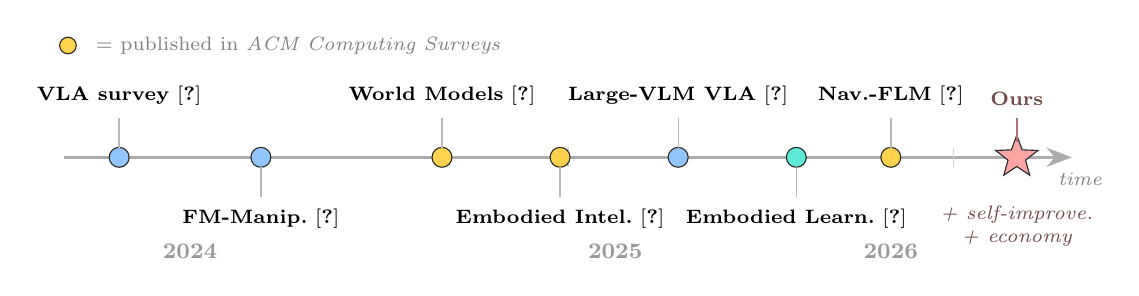
\begin{tikzpicture}[
  abv/.style={font=\scriptsize, anchor=south, align=center},
  blw/.style={font=\scriptsize, anchor=north, align=center},
  stem/.style={gray!55, line width=0.5pt},
]
\draw[-{Stealth[length=3.2mm]}, line width=1.3pt, gray!65] (-0.4,0) -- (12.4,0);
  \node[font=\scriptsize\itshape, gray, anchor=west] at (12.1,-0.28) {time};
\foreach \x in {0.3,6,10.9}{\draw[gray!35] (\x,-0.12) -- (\x,0.12);}
  \node[font=\footnotesize\bfseries,gray!80] at (1.2,-1.2) {2024};
  \node[font=\footnotesize\bfseries,gray!80] at (6.6,-1.2) {2025};
  \node[font=\footnotesize\bfseries,gray!80] at (10.1,-1.2) {2026};
\filldraw[fill=secD,draw=hidden-draw] (-0.35,1.42) circle (3pt);
  \node[font=\scriptsize,gray,anchor=west] at (-0.12,1.42) {= published in \emph{ACM Computing Surveys}};

\filldraw[fill=secA,draw=hidden-draw] (0.3,0) circle (3.6pt);
  \draw[stem] (0.3,0.12) -- (0.3,0.5);  \node[abv] at (0.3,0.53) {\textbf{VLA survey}~\cite{survey_vla}};

  \filldraw[fill=secA,draw=hidden-draw] (2.1,0) circle (3.6pt);
  \draw[stem] (2.1,-0.12) -- (2.1,-0.5); \node[blw] at (2.1,-0.53) {\textbf{FM-Manip.}~\cite{survey_fmrobot}};

  \filldraw[fill=secD,draw=hidden-draw] (4.4,0) circle (3.6pt);
  \draw[stem] (4.4,0.12) -- (4.4,0.5);  \node[abv] at (4.4,0.53) {\textbf{World Models}~\cite{survey_worldmodels}};

  \filldraw[fill=secD,draw=hidden-draw] (5.9,0) circle (3.6pt);
  \draw[stem] (5.9,-0.12) -- (5.9,-0.5); \node[blw] at (5.9,-0.53) {\textbf{Embodied Intel.}~\cite{survey_embodiedintel}};

  \filldraw[fill=secA,draw=hidden-draw] (7.4,0) circle (3.6pt);
  \draw[stem] (7.4,0.12) -- (7.4,0.5);  \node[abv] at (7.4,0.53) {\textbf{Large-VLM VLA}~\cite{survey_vlmvla}};

  \filldraw[fill=secB,draw=hidden-draw] (8.9,0) circle (3.6pt);
  \draw[stem] (8.9,-0.12) -- (8.9,-0.5); \node[blw] at (8.9,-0.53) {\textbf{Embodied Learn.}~\cite{survey_embodiedlearn}};

  \filldraw[fill=secD,draw=hidden-draw] (10.1,0) circle (3.6pt);
  \draw[stem] (10.1,0.12) -- (10.1,0.5); \node[abv] at (10.1,0.53) {\textbf{Nav.-FLM}~\cite{survey_navigation}};

\node[star,star points=5,star point ratio=2.4,fill=secE,draw=hidden-draw,minimum size=16pt,inner sep=0] at (11.7,0) {};
  \draw[secE!70!black,line width=0.6pt] (11.7,0.2) -- (11.7,0.5);
  \node[abv,text=secE!45!black] at (11.7,0.53) {\textbf{Ours}};
  \node[blw,text=secE!45!black,font=\scriptsize\itshape] at (11.7,-0.5) {+ self-improve.\\+ economy};
\end{tikzpicture}}
\caption{The closest related surveys as a timeline (2024--2026);
\textcolor{secD!55!black}{amber} markers denote surveys published in \emph{ACM Computing
Surveys} (CSUR). Prior surveys cover VLA models, foundation models, world models, and navigation,
but none organises code-as-policy by \emph{degree of self-improvement}. \textbf{Ours}
($\star$, 2026) is the first to add the self-improvement axis (\S3.1.5) and the skill economy;
per-topic coverage is in Table~\ref{tab:survey_compare}.}
\label{fig:surveys}
\end{figure}
 \FloatBarrier
 \section{A Taxonomy of Robot-Learning Techniques}
\label{sec:taxonomy}

Figure~\ref{fig:taxonomy_main} organizes the field into six branches. The dividing
question is \emph{what ships}: frozen weights (\S\ref{sec:vla}) or executable skills
(\S\ref{sec:code}). We tag mechanisms by \textbf{F}eedback, \textbf{S}earch, and
\textbf{M}emory throughout.

\begin{figure*}[tbp]
\centering
\resizebox{\textwidth}{!}{\begin{forest}
[\textbf{Robot-learning}\\\textbf{techniques for}\\\textbf{Physical AI}, fill=tx-root, text width=11em
  [\textbf{\S3.1 Code-as-policy for robots}, fill=cat-code, for descendants={fill=leaf-code}
    [\textbf{Code-as-Policies} --- LM programs for control~\citep{codeaspolicies}]
    [\textbf{ProgPrompt} --- situated task-plan programs~\citep{progprompt}]
    [\textbf{VoxPoser} --- composable 3D value maps~\citep{voxposer}]
    [\textbf{RoboCodeX} --- multimodal behavior code~\citep{robocodex}]
    [\textbf{Instruct2Act} --- instructions to action code~\citep{instruct2act}]
    [\textbf{RoboPro} --- video-instructed policy code~\citep{robopro}]
    [\textbf{RoboCoder} --- basic skills to general tasks~\citep{robocoder}]
    [\textbf{CaP-X} --- benchmarking robot coding agents~\citep{capx}]
    [\textbf{RoboClaw} --- scalable long-horizon agent~\citep{roboclaw}]
    [\textbf{ASPIRE}~$\star$ --- agentic skill discovery + self-improvement~\citep{aspire}]
    [\textbf{ENPIRE} --- real-world policy self-improvement~\citep{enpire}]
  ]
  [\textbf{\S3.2 End-to-end VLA / generalist policies}, fill=cat-vla, for descendants={fill=leaf-vla}
    [\textbf{RT-1} --- robotics transformer at scale~\citep{rt1}]
    [\textbf{RT-2} --- web knowledge to control~\citep{rt2}]
    [\textbf{Octo} --- open generalist policy~\citep{octo}]
    [\textbf{OpenVLA} --- open-source VLA~\citep{openvla}]
    [\textbf{RoboFlamingo} --- VLM robot imitator~\citep{roboflamingo}]
    [\textbf{CogACT} --- cognition + action VLA~\citep{cogact}]
    [\textbf{SpatialVLA} --- spatial-enhanced VLA~\citep{spatialvla}]
    [$\boldsymbol{\pi_0}$ --- VLA flow model~\citep{pi0}]
    [$\boldsymbol{\pi_{0.5}}$ --- open-world generalization~\citep{pi05}]
    [\textbf{GR00T N1} --- humanoid foundation model~\citep{groot}]
    [\textbf{Gemini Robotics} --- AI in the physical world~\citep{geminirobotics}]
  ]
  [\textbf{\S3.3 LLM-authored rewards / curricula}, fill=cat-rew, for descendants={fill=leaf-rew}
    [\textbf{Eureka} --- human-level reward design~\citep{eureka}]
    [\textbf{DrEureka} --- LLM-guided sim-to-real~\citep{dreureka}]
    [\textbf{Text2Reward} --- dense reward shaping~\citep{text2reward}]
    [\textbf{Language-to-Rewards} --- reward synthesis~\citep{l2r}]
    [\textbf{Eurekaverse} --- environment curriculum gen~\citep{eurekaverse}]
    [\textbf{RoboGen} --- generative task/skill learning~\citep{robogen}]
    [\textbf{Auto MC-Reward} --- automated dense rewards~\citep{automcreward}]
  ]
  [\textbf{\S3.4 Robot skill libraries \& lifelong learning}, fill=cat-skill, for descendants={fill=leaf-skill}
    [\textbf{Voyager} --- open-ended embodied agent~\citep{voyager}]
    [\textbf{LOTUS} --- unsupervised skill discovery~\citep{lotus}]
    [\textbf{LRLL} --- lifelong robot library learning~\citep{lrll}]
    [\textbf{BOSS} --- bootstrap your own skills~\citep{boss}]
    [\textbf{SPRINT} --- scalable skill pre-training~\citep{sprint}]
    [\textbf{Uni-Skill} --- self-evolving skill repository~\citep{uniskill}]
    [\textbf{SkillFlow} --- lifelong skill discovery~\citep{skillflow}]
  ]
  [\textbf{\S3.5 Sim-to-real \& cross-embodiment transfer}, fill=cat-trans, for descendants={fill=leaf-trans}
    [\textbf{Open X-Embodiment} --- RT-X cross-embodiment~\citep{openx}]
    [\textbf{CrossFormer} --- one policy many embodiments~\citep{crossformer}]
    [\textbf{RoboCat} --- self-improving generalist agent~\citep{robocat}]
    [\textbf{Mirage} --- zero-shot cross-embodiment transfer~\citep{mirage}]
  ]
  [\textbf{\S3.6 Embodied benchmarks \& simulators}, fill=cat-bench, for descendants={fill=leaf-bench}
    [\textbf{LIBERO} --- lifelong manipulation benchmark~\citep{libero}]
    [\textbf{Robosuite} --- modular sim framework~\citep{robosuite}]
    [\textbf{BEHAVIOR-1K} --- 1000 household activities~\citep{behavior1k}]
    [\textbf{Meta-World} --- 50-task multi-task RL~\citep{metaworld}]
    [\textbf{RLBench} --- 100-task robot learning~\citep{rlbench}]
    [\textbf{ManiSkill2} --- generalizable manipulation~\citep{maniskill2}]
    [\textbf{CALVIN} --- long-horizon language tasks~\citep{calvin}]
  ]
]
\end{forest}
}
\caption{Taxonomy of robot-learning techniques for Physical AI ($\sim$47 systems).
The fault line: \S3.1 ships \emph{code} and \S3.2 ships \emph{weights}.
\textbf{ASPIRE}~$\star$ anchors the self-improving code-as-policy frontier (\S\ref{sec:code}).}
\label{fig:taxonomy_main}
\end{figure*}
 
Table~\ref{tab:compare_main} compares all systems in the map on what each \emph{ships}, where
it is evaluated, and whether it improves from its own experience.
{\footnotesize
\begin{longtable}{@{}p{0.30\textwidth}cll c c@{}}
\caption{Comparison of all $\sim$47 systems in the main taxonomy (Figure~\ref{fig:taxonomy_main}),
grouped by family. \textbf{Ships}: \tcode/\tweights/\treward/\tskill/\tpolicy/\tbench.
\textbf{Eval}: \dreal/\dsim/\dgame. \textbf{Self-impr.}: \yy\ learns from its own experience,
\pp\ partially, \nn\ no, \dm\ n/a.}\label{tab:compare_main}\\
\toprule
\textbf{System} & \textbf{Year} & \textbf{Venue} & \textbf{Ships} & \textbf{Eval} & \textbf{Self-impr.}\\
\midrule
\endfirsthead
\multicolumn{6}{@{}l}{\footnotesize\emph{Table~\ref{tab:compare_main} (continued)}}\\
\toprule
\textbf{System} & \textbf{Year} & \textbf{Venue} & \textbf{Ships} & \textbf{Eval} & \textbf{Self-impr.}\\
\midrule
\endhead
\bottomrule
\endlastfoot
\multicolumn{6}{@{}l}{\textbf{\S3.1 Code-as-policy for robots} \hfill \tcode}\\
\textbf{Code-as-Policies}~\cite{codeaspolicies} & 2023 & ICRA & \tcode & \dreal & \nn\\
\textbf{ProgPrompt}~\cite{progprompt} & 2023 & ICRA & \tcode & \dreal & \nn\\
\textbf{VoxPoser}~\cite{voxposer} & 2023 & CoRL & \tcode & \dreal & \nn\\
\textbf{RoboCodeX}~\cite{robocodex} & 2024 & ICML & \tcode & \dsim & \nn\\
\textbf{Instruct2Act}~\cite{instruct2act} & 2023 & arXiv & \tcode & \dsim & \nn\\
\textbf{RoboPro}~\cite{robopro} & 2025 & arXiv & \tcode & \dreal & \nn\\
\textbf{RoboCoder}~\cite{robocoder} & 2024 & arXiv & \tcode & \dsim & \nn\\
\textbf{CaP-X}~\cite{capx} & 2026 & arXiv & \tcode & \dsim & \yy\\
\textbf{RoboClaw}~\cite{roboclaw} & 2026 & arXiv & \tcode & \dreal & \yy\\
\textbf{ASPIRE}~\cite{aspire} & 2026 & arXiv & \tcode & \dreal & \yy\\
\textbf{ENPIRE}~\cite{enpire} & 2026 & arXiv & \tcode & \dreal & \yy\\
\midrule
\multicolumn{6}{@{}l}{\textbf{\S3.2 End-to-end VLA / generalist policies} \hfill \tweights}\\
\textbf{RT-1}~\cite{rt1} & 2023 & RSS & \tweights & \dreal & \nn\\
\textbf{RT-2}~\cite{rt2} & 2023 & CoRL & \tweights & \dreal & \nn\\
\textbf{Octo}~\cite{octo} & 2024 & RSS & \tweights & \dreal & \nn\\
\textbf{OpenVLA}~\cite{openvla} & 2024 & CoRL & \tweights & \dreal & \nn\\
\textbf{RoboFlamingo}~\cite{roboflamingo} & 2024 & ICLR & \tweights & \dsim & \nn\\
\textbf{CogACT}~\cite{cogact} & 2024 & arXiv & \tweights & \dreal & \nn\\
\textbf{SpatialVLA}~\cite{spatialvla} & 2025 & arXiv & \tweights & \dreal & \nn\\
$\boldsymbol{\pi_0}$~\cite{pi0} & 2024 & arXiv & \tweights & \dreal & \nn\\
$\boldsymbol{\pi_{0.5}}$~\cite{pi05} & 2025 & arXiv & \tweights & \dreal & \nn\\
\textbf{GR00T N1}~\cite{groot} & 2025 & arXiv & \tweights & \dreal & \nn\\
\textbf{Gemini Robotics}~\cite{geminirobotics} & 2025 & arXiv & \tweights & \dreal & \nn\\
\midrule
\multicolumn{6}{@{}l}{\textbf{\S3.3 LLM-authored rewards / curricula} \hfill \treward}\\
\textbf{Eureka}~\cite{eureka} & 2024 & ICLR & \treward & \dsim & \yy\\
\textbf{DrEureka}~\cite{dreureka} & 2024 & RSS & \treward & \dreal & \yy\\
\textbf{Text2Reward}~\cite{text2reward} & 2024 & ICLR & \treward & \dsim & \pp\\
\textbf{Language-to-Rewards}~\cite{l2r} & 2023 & CoRL & \treward & \dreal & \pp\\
\textbf{Eurekaverse}~\cite{eurekaverse} & 2024 & CoRL & \treward & \dsim & \yy\\
\textbf{RoboGen}~\cite{robogen} & 2024 & ICML & \treward & \dsim & \yy\\
\textbf{Auto MC-Reward}~\cite{automcreward} & 2024 & CVPR & \treward & \dgame & \yy\\
\midrule
\multicolumn{6}{@{}l}{\textbf{\S3.4 Robot skill libraries \& lifelong learning} \hfill \tskill}\\
\textbf{Voyager}~\cite{voyager} & 2023 & arXiv & \tskill & \dgame & \yy\\
\textbf{LOTUS}~\cite{lotus} & 2024 & ICRA & \tskill & \dsim & \yy\\
\textbf{LRLL}~\cite{lrll} & 2024 & ICRA & \tskill & \dsim & \yy\\
\textbf{BOSS}~\cite{boss} & 2023 & CoRL & \tskill & \dsim & \yy\\
\textbf{SPRINT}~\cite{sprint} & 2024 & ICRA & \tskill & \dsim & \pp\\
\textbf{Uni-Skill}~\cite{uniskill} & 2026 & ICRA & \tskill & \dreal & \yy\\
\textbf{SkillFlow}~\cite{skillflow} & 2026 & arXiv & \tskill & \dtext & \yy\\
\midrule
\multicolumn{6}{@{}l}{\textbf{\S3.5 Sim-to-real \& cross-embodiment transfer} \hfill \tpolicy}\\
\textbf{Open X-Embodiment}~\cite{openx} & 2024 & ICRA & \tpolicy & \dreal & \nn\\
\textbf{CrossFormer}~\cite{crossformer} & 2024 & CoRL & \tpolicy & \dreal & \nn\\
\textbf{RoboCat}~\cite{robocat} & 2023 & TMLR & \tpolicy & \dreal & \yy\\
\textbf{Mirage}~\cite{mirage} & 2024 & RSS & \tpolicy & \dreal & \nn\\
\midrule
\multicolumn{6}{@{}l}{\textbf{\S3.6 Embodied benchmarks \& simulators} \hfill \tbench}\\
\textbf{LIBERO}~\cite{libero} & 2023 & NeurIPS & \tbench & \dsim & \dm\\
\textbf{Robosuite}~\cite{robosuite} & 2020 & arXiv & \tbench & \dsim & \dm\\
\textbf{BEHAVIOR-1K}~\cite{behavior1k} & 2024 & arXiv & \tbench & \dsim & \dm\\
\textbf{Meta-World}~\cite{metaworld} & 2019 & CoRL & \tbench & \dsim & \dm\\
\textbf{RLBench}~\cite{rlbench} & 2020 & RA-L & \tbench & \dsim & \dm\\
\textbf{ManiSkill2}~\cite{maniskill2} & 2023 & ICLR & \tbench & \dsim & \dm\\
\textbf{CALVIN}~\cite{calvin} & 2022 & RA-L & \tbench & \dsim & \dm\\
\end{longtable}
}
  \section{The Technique Families}
\label{sec:techniques}

We now examine each of the six branches of the taxonomy (Figure~\ref{fig:taxonomy_main}) in
turn. We begin with the code-as-policy camp (\S\ref{sec:code})---the focus of this survey and
the only family we organise by \emph{degree of self-improvement}---and then survey the
weights-based (\S\ref{sec:vla}), reward-synthesis (\S\ref{sec:reward}), skill-library
(\S\ref{sec:skill}), transfer (\S\ref{sec:transfer}), and benchmark (\S\ref{sec:bench})
families that surround it.
 \subsection{Code-as-Policy: Robots that Write their Own Skills}
\label{sec:code}

The organising contribution of this survey is to arrange code-as-policy methods not by
application or robot embodiment, but by \emph{how much of their own competence a system
produces at run time}. Concretely, we ask five questions in sequence: does the agent (i)
write control code at all, (ii) repair that code from execution feedback within a task,
(iii) remember validated code across tasks, (iv) search a population of programs rather
than following a single trajectory of repairs, and (v) close all of these into one
open-ended loop? Each ``yes'' is a rung on the ladder of Figure~\ref{fig:taxonomy_31}, and
the population thins sharply toward the top: of the thirteen zero-shot systems, only a
handful ever reach the combined feedback--memory--search regime. The novelty of the
survey is naming this progression and showing that the top rung is nearly empty.

\begin{figure*}[tbp]
\centering
\resizebox{\textwidth}{!}{\begin{forest}
[\textbf{\S3.1 Code-as-policy}\\\textbf{ordered by how much a}\\\textbf{system improves itself}, fill=tx-root, text width=12em
  [{\textbf{\S3.1.1 Zero-shot synthesis} (n=13)\\\emph{write once, no learning from execution}}, fill=secA, text width=19em, for descendants={fill=secAl, text width=26em}
    [\textbf{Code-as-Policies}~\citep{codeaspolicies}]
    [\textbf{ProgPrompt}~\citep{progprompt}]
    [\textbf{VoxPoser}~\citep{voxposer}]
    [\textbf{Instruct2Act}~\citep{instruct2act}]
    [\textbf{ChatGPT for Robotics}~\citep{chatgptrobotics}]
    [\textbf{TidyBot}~\citep{tidybot}]
    [\textbf{RoboCodeX}~\citep{robocodex}]
    [\textbf{RoboScript}~\citep{roboscript}]
    [\textbf{Text2Motion}~\citep{text2motion}]
    [\textbf{Demo2Code}~\citep{demo2code}]
    [\textbf{Statler}~\citep{statler}]
    [\textbf{Prompt2Walk}~\citep{prompt2walk}]
    [\textbf{RoboPro}~\citep{robopro}]
  ]
  [{\textbf{\S3.1.2 Closed-loop self-repair} (n=6)\\\emph{detect \& fix failures from feedback}}, fill=secB, text width=19em, for descendants={fill=secBl, text width=26em}
    [\textbf{Inner Monologue}~\citep{innermonologue}]
    [\textbf{DoReMi}~\citep{doremi}]
    [\textbf{REFLECT}~\citep{reflect}]
    [\textbf{Code-as-Monitor}~\citep{codeasmonitor}]
    [\textbf{AHA}~\citep{aha}]
    [\textbf{Introspective Planning}~\citep{introspective}]
  ]
  [{\textbf{\S3.1.3 Skill-library accumulation} (n=5)\\\emph{the memory step}}, fill=secC, text width=19em, for descendants={fill=secCl, text width=40em}
    [{code skill libraries $\rightarrow$ cataloged once in \textbf{\S3.4.3} (Voyager, LRLL, RoboCoder, Uni-Skill, DROC)}]
  ]
  [{\textbf{\S3.1.4 Evolutionary program search} (n=3)\\\emph{search a population, not one repair}}, fill=secD, text width=19em, for descendants={fill=secDl, text width=26em}
    [\textbf{CaP-X}~\citep{capx}]
    [\textbf{RoboEvolve}~\citep{roboevolve}]
    [\textbf{GEAR (code evolution)}~\citep{codeevolution}]
  ]
  [{\textbf{\S3.1.5 Full self-improving loop} (n=3)\\\emph{the gap: feedback + memory + search}}, fill=secE, text width=19em, for descendants={fill=secEl, text width=26em}
    [\textbf{ASPIRE}~$\star$~\citep{aspire}]
    [\textbf{ENPIRE}~\citep{enpire}]
    [\textbf{RoboClaw}~\citep{roboclaw}]
  ]
]
\end{forest}
}
\caption{The self-improvement funnel within code-as-policy ($13\!\to\!6\!\to\!5\!\to\!3\!\to\!3$),
one colour per sub-section. As the demand rises (write once $\to$ repair $\to$ remember $\to$
search $\to$ all three), occupants thin out; \S3.1.5---feedback $+$ memory $+$ search
combined---is nearly empty, and only \textbf{ASPIRE}~$\star$ was built for it end-to-end.}
\label{fig:taxonomy_31}
\end{figure*}
 \begin{figure}[t]
\centering
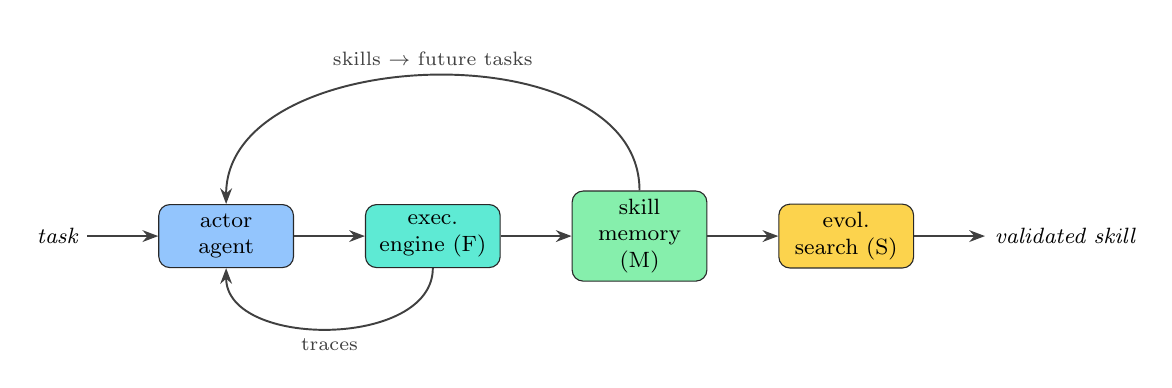
\begin{tikzpicture}[
  node distance=6mm and 9mm,
  box/.style={draw=hidden-draw, rounded corners, fill=secAl, align=center,
              font=\footnotesize, minimum height=8mm, text width=15mm, inner sep=3pt},
  core/.style={box, fill=secA},
  io/.style={draw=none, font=\footnotesize\itshape},
  ar/.style={-{Stealth[length=2mm]}, darkgray, line width=0.7pt},
]
  \node[io] (task) {task};
  \node[box, fill=secA, right=of task] (actor) {actor\\ agent};
  \node[box, fill=secB, right=of actor] (eng) {exec.\\ engine (F)};
  \node[box, fill=secC, right=of eng] (mem) {skill\\ memory (M)};
  \node[box, fill=secD, right=of mem] (srch) {evol.\\ search (S)};
  \node[io, right=of srch] (out) {validated skill};

  \draw[ar] (task) -- (actor);
  \draw[ar] (actor) -- (eng);
  \draw[ar] (eng) -- (mem);
  \draw[ar] (mem) -- (srch);
  \draw[ar] (srch) -- (out);
\draw[ar] (eng.south) to[out=-90,in=-90] node[below,font=\scriptsize]{traces} (actor.south);
  \draw[ar] (mem.north) to[out=90,in=90] node[above,font=\scriptsize]{skills $\rightarrow$ future tasks} (actor.north);
\end{tikzpicture}
\caption{The full self-improving loop (\S3.1.5): feedback (F) $+$ memory (M) $+$ search (S)
combine into one open-ended loop---the ASPIRE cell. VLAs (\S3.2) have no such loop.}
\label{fig:architectures}
\end{figure}
 
\subsubsection{Zero-shot synthesis}
\label{ssec:zeroshot}
The foundational move is to treat the language model as a \emph{program synthesiser} over
a fixed library of perception and control primitives. \emph{Code-as-Policies}
\citep{codeaspolicies} showed that an LLM prompted with an API and a natural-language
instruction can emit executable Python that composes those primitives, recursively
defining undefined functions and parameterising control with arithmetic and feedback
logic. \emph{ProgPrompt} \citep{progprompt} situates the generated program in the scene
by exposing available actions and objects as importable symbols, while \emph{VoxPoser}
\citep{voxposer} has the model write code that \emph{composes 3D value maps} for a motion
planner rather than calling fixed skills, loosening the dependence on a hand-authored API.
Subsequent work broadened the input modality and task horizon---\emph{RoboCodeX}
\citep{robocodex} conditions on multimodal observations, \emph{Instruct2Act}
\citep{instruct2act} maps instructions to perception--action code, and video- and
demonstration-conditioned variants such as \emph{RoboPro} \citep{robopro},
\emph{Demo2Code} \citep{demo2code} and \emph{Text2Motion} \citep{text2motion} recover
programs from richer context. \emph{Statler} \citep{statler} maintains an explicit world
state across steps, and \emph{TidyBot} \citep{tidybot} and \emph{ChatGPT for Robotics}
\citep{chatgptrobotics} demonstrate personalisation and prompt design for real hardware.
What unites this rung, and limits it, is that the program is written \emph{once}: there is
no channel from execution back to the synthesiser, so a plan that fails at run time simply
fails.

\subsubsection{Closed-loop self-repair}
\label{ssec:selfrepair}
The second rung adds a within-task feedback loop. \emph{Inner Monologue}
\citep{innermonologue} feeds success detectors, scene descriptions and human feedback back
into the model as language, letting it replan when a step fails. \emph{DoReMi}
\citep{doremi} detects misalignments between plan and execution and triggers recovery, and
\emph{REFLECT} \citep{reflect} builds a hierarchical, multimodal summary of past
interaction that an LLM queries to explain a failure and propose a correction. More recent
systems push the monitor into the perception loop---\emph{Code-as-Monitor}
\citep{codeasmonitor} compiles spatio-temporal constraints into vision-language checks, and
\emph{AHA} \citep{aha} trains a model to reason explicitly about failure modes. The novelty
of this rung is the closed loop, but it is a \emph{short} loop: corrections are discarded
at task boundaries, so nothing accumulates.

\subsubsection{Skill-library accumulation}
\label{ssec:skilllib}
The third rung makes the loop persistent by writing validated code into a growing library
that later tasks retrieve and compose. Because this ``memory'' axis is a full technique
family in its own right, we catalogue its systems once, in \S\ref{sec:skill}
(\S3.4.3)---\emph{Voyager} \citep{voyager} is the canonical example, curating an
ever-growing library of verified skill programs with when-to-apply guards, while related
methods distil language corrections into retrievable knowledge for future tasks~\citep{droc}. The key
distinction from \S3.1.2 is temporal scope: competence compounds \emph{across} tasks rather
than being rebuilt each time.

\subsubsection{Evolutionary program search}
\label{ssec:search}
The fourth rung replaces a single chain of repairs with population-based search over
programs. Rather than iteratively debugging one candidate, the agent maintains several,
scores them by execution, and mutates the best. \emph{CaP-X} \citep{capx} provides an
interactive gym and benchmark for exactly this style of coding agent, and \emph{RoboEvolve}
\citep{roboevolve} couples a planner and a learned simulator into a co-evolutionary loop
that mines near-miss failures to stabilise search. The novelty is the shift from
\emph{repair} to \emph{search}: exploration is explicit and parallel, which trades compute
for a better chance of escaping local failures.

\subsubsection{The full self-improving loop}
\label{ssec:fullloop}
The top rung combines all three mechanisms---execution feedback (F), a persistent skill
memory (M), and evolutionary search (S)---into one open-ended loop
(Figure~\ref{fig:architectures}). \emph{ASPIRE} \citep{aspire} instantiates this with a
robot execution engine that emits per-primitive multimodal traces, a skill library of
validated code with guards, and a population search over candidate programs, so that
experience compounds and transfers across tasks and embodiments. Its real-world sibling
\emph{ENPIRE} \citep{enpire} closes the same loop on physical hardware, using automatic
reset, parallel rollouts, and log-driven algorithm revision to drive a coding agent to
near-perfect success on dexterous tasks. This cell---feedback \emph{and} memory \emph{and}
search---is what no prior survey isolates, and it is nearly empty; it is the central gap this survey is organised to expose.

Table~\ref{tab:compare_31} makes the funnel explicit, tabulating each system's use of
feedback (F), memory (M), and search (S).
{\footnotesize
\begin{longtable}{@{}p{0.36\textwidth}c ccc c@{}}
\caption{The 30 code-as-policy systems of Figure~\ref{fig:taxonomy_31} on the three
self-improvement mechanisms---\textbf{F}eedback, \textbf{M}emory, \textbf{S}earch---which are
determined by the rung. \yy\ present, \nn\ absent. \textbf{Self-impr.}: \yy\ full loop,
\pp\ partial, \nn\ none.}\label{tab:compare_31}\\
\toprule
\textbf{System} & \textbf{Year} & \textbf{F} & \textbf{M} & \textbf{S} & \textbf{Self-impr.}\\
\midrule
\endfirsthead
\multicolumn{6}{@{}l}{\footnotesize\emph{Table~\ref{tab:compare_31} (continued)}}\\
\toprule
\textbf{System} & \textbf{Year} & \textbf{F} & \textbf{M} & \textbf{S} & \textbf{Self-impr.}\\
\midrule
\endhead
\bottomrule
\endlastfoot
\multicolumn{6}{@{}l}{\textbf{\S3.1.1 Zero-shot synthesis} \hfill F\,\nn\ \ M\,\nn\ \ S\,\nn}\\
\textbf{Code-as-Policies}~\cite{codeaspolicies} & 2023 & \nn & \nn & \nn & \nn\\
\textbf{ProgPrompt}~\cite{progprompt} & 2023 & \nn & \nn & \nn & \nn\\
\textbf{VoxPoser}~\cite{voxposer} & 2023 & \nn & \nn & \nn & \nn\\
\textbf{Instruct2Act}~\cite{instruct2act} & 2023 & \nn & \nn & \nn & \nn\\
\textbf{ChatGPT for Robotics}~\cite{chatgptrobotics} & 2023 & \nn & \nn & \nn & \nn\\
\textbf{TidyBot}~\cite{tidybot} & 2023 & \nn & \nn & \nn & \nn\\
\textbf{RoboCodeX}~\cite{robocodex} & 2024 & \nn & \nn & \nn & \nn\\
\textbf{RoboScript}~\cite{roboscript} & 2024 & \nn & \nn & \nn & \nn\\
\textbf{Text2Motion}~\cite{text2motion} & 2023 & \nn & \nn & \nn & \nn\\
\textbf{Demo2Code}~\cite{demo2code} & 2023 & \nn & \nn & \nn & \nn\\
\textbf{Statler}~\cite{statler} & 2024 & \nn & \nn & \nn & \nn\\
\textbf{Prompt2Walk}~\cite{prompt2walk} & 2024 & \nn & \nn & \nn & \nn\\
\textbf{RoboPro}~\cite{robopro} & 2025 & \nn & \nn & \nn & \nn\\
\midrule
\multicolumn{6}{@{}l}{\textbf{\S3.1.2 Closed-loop self-repair} \hfill F\,\yy\ \ M\,\nn\ \ S\,\nn}\\
\textbf{Inner Monologue}~\cite{innermonologue} & 2022 & \yy & \nn & \nn & \nn\\
\textbf{DoReMi}~\cite{doremi} & 2024 & \yy & \nn & \nn & \nn\\
\textbf{REFLECT}~\cite{reflect} & 2023 & \yy & \nn & \nn & \nn\\
\textbf{Code-as-Monitor}~\cite{codeasmonitor} & 2025 & \yy & \nn & \nn & \nn\\
\textbf{AHA}~\cite{aha} & 2024 & \yy & \nn & \nn & \nn\\
\textbf{Introspective Planning}~\cite{introspective} & 2024 & \yy & \nn & \nn & \nn\\
\midrule
\multicolumn{6}{@{}l}{\textbf{\S3.1.3 Skill-library accumulation} \hfill F\,\nn\ \ M\,\yy\ \ S\,\nn}\\
\textbf{Voyager}~\cite{voyager} & 2023 & \nn & \yy & \nn & \pp\\
\textbf{LRLL}~\cite{lrll} & 2024 & \nn & \yy & \nn & \pp\\
\textbf{RoboCoder}~\cite{robocoder} & 2024 & \nn & \yy & \nn & \pp\\
\textbf{Uni-Skill}~\cite{uniskill} & 2026 & \nn & \yy & \nn & \pp\\
\textbf{DROC}~\cite{droc} & 2024 & \yy & \yy & \nn & \pp\\
\midrule
\multicolumn{6}{@{}l}{\textbf{\S3.1.4 Evolutionary program search} \hfill F\,\yy\ \ M\,\nn\ \ S\,\yy}\\
\textbf{CaP-X}~\cite{capx} & 2026 & \yy & \nn & \yy & \pp\\
\textbf{RoboEvolve}~\cite{roboevolve} & 2026 & \yy & \nn & \yy & \pp\\
\textbf{Code Evolution (GEAR)}~\cite{codeevolution} & 2026 & \yy & \nn & \yy & \pp\\
\midrule
\multicolumn{6}{@{}l}{\textbf{\S3.1.5 Full self-improving loop} \hfill F\,\yy\ \ M\,\yy\ \ S\,\yy}\\
\textbf{ASPIRE}~\cite{aspire} & 2026 & \yy & \yy & \yy & \yy\\
\textbf{ENPIRE}~\cite{enpire} & 2026 & \yy & \yy & \yy & \yy\\
\textbf{RoboClaw}~\cite{roboclaw} & 2026 & \yy & \yy & \yy & \yy\\
\end{longtable}
}
  \subsection{End-to-End Vision-Language-Action Models}
\label{sec:vla}

The dominant alternative to writing code is to regress actions directly from pixels and
language with a single large network, so that competence lives in \emph{frozen weights}
rather than in an inspectable program. Architecturally these vision-language-action (VLA)
models share a backbone--action-head decomposition: a vision-language backbone encodes the
scene and instruction, and a pluggable action head maps that representation to motor
commands~\citep{openvla,pi0}.

The lineage begins with \emph{RT-1}~\citep{rt1}, a transformer trained on large-scale real
robot data that discretises continuous actions into categorical bins. \emph{RT-2}~\citep{rt2}
then co-fine-tunes an Internet-pretrained vision-language model on robot trajectories,
emitting actions as text tokens and inheriting semantic generalisation from web data. Open
reproductions followed: \emph{Octo}~\citep{octo} and \emph{OpenVLA}~\citep{openvla}---the
latter a 7B model with a DINOv2/SigLIP vision stack---are trained on the pooled
Open X-Embodiment corpus (\S\ref{sec:transfer}), and \emph{RoboFlamingo}~\citep{roboflamingo}
adapts a vision-language model into an imitation policy.

A second design axis is the \emph{action representation}. Discrete token heads (RT-1/RT-2)
are simple but coarse; recent systems favour continuous heads. \emph{$\pi_0$}~\citep{pi0}
attaches a \emph{flow-matching} head to a PaLI-Gemma backbone for smooth, high-frequency
bimanual control, and \emph{$\pi_{0.5}$}~\citep{pi05} extends it toward open-world
generalisation; \emph{CogACT}~\citep{cogact} separates a cognition module from a
diffusion-transformer action module, and \emph{SpatialVLA}~\citep{spatialvla} injects 3D
spatial encodings. Flow- and diffusion-based heads trade a few extra parameters for far fewer
inference steps and better high-degree-of-freedom precision.

At the largest scale, foundation-model efforts target whole platforms:
\emph{GR00T~N1}~\citep{groot} pairs a slow System-2 vision-language reasoner with a fast
System-1 diffusion transformer that produces motor actions at high rate for humanoids, and
\emph{Gemini Robotics}~\citep{geminirobotics} builds a VLA together with an embodied-reasoning
model on the Gemini backbone. Across all of these, the defining property---and the reason we
treat them as the \emph{foil} for this survey---is that there is \emph{no loop and no code}:
competence is acquired by scaling data and parameters, generalises by interpolation rather
than search, and cannot be edited, audited, or recombined after training.
 \subsection{Reward and Curriculum Synthesis}
\label{sec:reward}

A third family keeps the language model in the role of programmer but points it at a
different artefact: instead of policy code, it writes the \emph{reward}, \emph{environment},
or \emph{curriculum} that a reinforcement-learning loop then compiles into a policy. A
feedback loop exists---the model reads back training statistics and revises---but what ships
is still weights, which is why we separate this family from the self-improving code camp
(\S\ref{sec:code}).

\emph{Eureka}~\citep{eureka} is the canonical instance: given unmodified environment source
code and a task description, a coding LLM zero-shot generates an executable reward function,
then improves it by \emph{evolutionary search} guided by \emph{reward reflection}---a textual
summary of training statistics---exceeding expert human rewards on 83\% of a 29-task IsaacGym
suite. \emph{DrEureka}~\citep{dreureka} extends the idea to sim-to-real by also synthesising
domain-randomisation ranges, achieving zero-shot real-world locomotion.
\emph{Text2Reward}~\citep{text2reward} generates dense reward programs grounded in a compact
environment representation and refines them from human feedback, matching or beating
expert-written rewards on most of a seventeen-task suite, while \emph{Language to
Rewards}~\citep{l2r} uses the reward function as the interface between an LLM and a MuJoCo
model-predictive controller.

Beyond the reward itself, the same generative recipe is applied to the \emph{training
environment}. \emph{Eurekaverse}~\citep{eurekaverse} has an LLM propose a progressively harder
curriculum of environments---learning parkour skills that transfer to a real robot---and
\emph{RoboGen}~\citep{robogen} runs a propose-generate-learn cycle that fabricates tasks,
scenes, and supervision in simulation to unlock effectively unlimited training data;
\emph{Auto MC-Reward}~\citep{automcreward} automates dense rewards for open-world Minecraft.
The through-line is that language becomes a bridge from high-level intent to low-level control
\emph{via} an RL optimiser, rather than producing an executable, reusable skill directly.
 \subsection{Skill Libraries: How a Repertoire is Built}
\label{sec:skill}

Where \S\ref{sec:code} asked \emph{how} a code skill improves, this family asks the prior
question of \emph{how a repertoire of skills is built at all}. Figure~\ref{fig:taxonomy_34}
organises the answer along one axis---skills learned as latent reinforcement-learning policies
versus skills stored as retrievable code---and only the code flavour self-improves without
gradients, which links this family back to \S\ref{sec:code}.

\begin{figure*}[tbp]
\centering
\resizebox{\textwidth}{!}{\begin{forest}
[\textbf{\S3.4 Robot skills}\\\textbf{how a repertoire is}\\\textbf{built \& reused}, fill=tx-root, text width=11em
  [{\textbf{\S3.4.1 Unsupervised / latent discovery} (RL)\\\emph{diverse skills, no reward, no code}}, fill=secA, text width=19em, for descendants={fill=secAl, text width=33em}
    [\textbf{DIAYN} --- diversity is all you need~\citep{diayn}]
    [\textbf{DADS} --- dynamics-aware skills~\citep{dads}]
    [\textbf{LSD} --- Lipschitz skill discovery~\citep{lsd}]
    [\textbf{CIC} --- contrastive intrinsic control~\citep{cic}]
    [\textbf{METRA} --- metric-aware abstraction~\citep{metra}]
  ]
  [{\textbf{\S3.4.2 Skill-based / hierarchical RL}\\\emph{learn a skill space, then compose}}, fill=secB, text width=19em, for descendants={fill=secBl, text width=33em}
    [\textbf{SPiRL} --- learned skill priors~\citep{spirl}]
    [\textbf{OPAL} --- offline primitive discovery~\citep{opal}]
    [\textbf{PARROT} --- behavioral priors~\citep{parrot}]
    [\textbf{SkiMo} --- skill-based model-based RL~\citep{skimo}]
  ]
  [{\textbf{\S3.4.3 LLM / code skill libraries}\\\emph{skills as retrievable code (ASPIRE lives here)}}, fill=secF, text width=19em, for descendants={fill=secFl, text width=33em}
    [\textbf{Voyager} --- open-ended embodied agent~\citep{voyager}]
    [\textbf{LOTUS} --- unsupervised skill discovery~\citep{lotus}]
    [\textbf{LRLL} --- lifelong robot library learning~\citep{lrll}]
    [\textbf{BOSS} --- bootstrap your own skills~\citep{boss}]
    [\textbf{SPRINT} --- scalable skill pre-training~\citep{sprint}]
    [\textbf{Uni-Skill} --- self-evolving skill repository~\citep{uniskill}]
    [\textbf{SkillFlow} --- lifelong skill discovery~\citep{skillflow}]
  ]
  [{\textbf{\S3.4.4 Open-world LLM-agent libraries}\\\emph{agents build \& reuse from experience}}, fill=secG, text width=19em, for descendants={fill=secGl, text width=33em}
    [\textbf{GITM} --- Ghost in the Minecraft~\citep{gitm}]
    [\textbf{JARVIS-1} --- memory-augmented agent~\citep{jarvis1}]
    [\textbf{ExpeL} --- experiential learner~\citep{expel}]
    [\textbf{Optimus-1} --- hybrid multimodal memory~\citep{optimus1}]
    [\textbf{Odyssey} --- open-world skill library~\citep{odyssey}]
  ]
]
\end{forest}
}
\caption{The ``skills'' pole, one colour per sub-section. \S3.4.1--2 build skills as
\emph{RL policies} (mature, included as landscape); \S3.4.3--4 build them as
\emph{retrievable code}, where ASPIRE's self-improving \S3.1 lives.}
\label{fig:taxonomy_34}
\end{figure*}
 
\subsubsection{Unsupervised and latent skill discovery}
The oldest lineage learns a diverse set of skills with \emph{no task reward and no code}, by
maximising an information-theoretic objective. \emph{DIAYN}~\citep{diayn} maximises the mutual
information between a latent skill code and the visited states, yielding distinguishable
behaviours; \emph{DADS}~\citep{dads} makes the discovered skills dynamics-aware and hence
usable for model-based control; and \emph{LSD}~\citep{lsd}, \emph{CIC}~\citep{cic}, and
\emph{METRA}~\citep{metra} push toward more dynamic, far-reaching, and scalable skills through
Lipschitz constraints, contrastive objectives, and metric-aware abstractions respectively.

\subsubsection{Skill-based and hierarchical reinforcement learning}
A second lineage extracts a continuous \emph{skill space} from offline data and then plans or
learns within it. \emph{SPiRL}~\citep{spirl} learns a skill embedding together with a skill
prior that accelerates downstream RL; \emph{OPAL}~\citep{opal} discovers temporally extended
primitives for offline RL; \emph{PARROT}~\citep{parrot} learns an invertible behavioural
prior; and \emph{SkiMo}~\citep{skimo} learns a skill dynamics model so that planning happens
directly in skill space.

\subsubsection{LLM and code skill libraries}
The code flavour---where the self-improving methods of \S\ref{sec:code} live---stores skills as
retrievable programs. \emph{Voyager}~\citep{voyager} curates an ever-growing library of
verified code skills in Minecraft; \emph{LOTUS}~\citep{lotus} performs continual imitation
learning through unsupervised skill discovery; \emph{LRLL}~\citep{lrll} bootstraps a composable
robot library with language models; and \emph{BOSS}~\citep{boss} and \emph{SPRINT}~\citep{sprint}
grow skill repertoires by LLM-guided bootstrapping and instruction relabelling. The most recent
entries close the loop between video and code: \emph{Uni-Skill}~\citep{uniskill} builds a
self-evolving skill repository from unstructured robot video, and \emph{SkillFlow}~\citep{skillflow}
benchmarks lifelong discovery, patching, and reuse of a skill library.

\subsubsection{Open-world LLM-agent libraries}
Finally, embodied LLM agents accumulate skills from open-ended experience.
\emph{GITM}~\citep{gitm} and \emph{JARVIS-1}~\citep{jarvis1} pair a planner with text or
multimodal memory in Minecraft; \emph{ExpeL}~\citep{expel} extracts reusable insights from a
stream of trials; \emph{Optimus-1}~\citep{optimus1} adds a hybrid multimodal memory for
long-horizon tasks; and \emph{Odyssey}~\citep{odyssey} equips an agent with an open-world
library of primitive and compositional skills. These systems foreshadow the marketplace
dynamics of \S\ref{sec:open}: a library that grows with use.

Table~\ref{tab:compare_34} contrasts the four sub-families on skill form, whether they are
gradient-trained or LLM-authored, whether they keep a persistent library, and their domain.
{\footnotesize
\begin{longtable}{@{}p{0.30\textwidth}c l c c c@{}}
\caption{The 21 skill-building systems of Figure~\ref{fig:taxonomy_34}, by sub-family.
\textbf{Form}: \flatent/\fspace/\fcodelib/\fagent. \textbf{Grad.}: gradient-trained (\yy) vs
LLM-authored (\nn). \textbf{Lib.}: persistent retrievable library. \textbf{Domain}:
\dsim/\dgame/\dreal/\dtext.}\label{tab:compare_34}\\
\toprule
\textbf{System} & \textbf{Year} & \textbf{Form} & \textbf{Grad.} & \textbf{Lib.} & \textbf{Domain}\\
\midrule
\endfirsthead
\multicolumn{6}{@{}l}{\footnotesize\emph{Table~\ref{tab:compare_34} (continued)}}\\
\toprule
\textbf{System} & \textbf{Year} & \textbf{Form} & \textbf{Grad.} & \textbf{Lib.} & \textbf{Domain}\\
\midrule
\endhead
\bottomrule
\endlastfoot
\multicolumn{6}{@{}l}{\textbf{\S3.4.1 Unsupervised / latent discovery (RL)}}\\
\textbf{DIAYN}~\cite{diayn} & 2019 & \flatent & \yy & \nn & \dsim\\
\textbf{DADS}~\cite{dads} & 2020 & \flatent & \yy & \nn & \dsim\\
\textbf{LSD}~\cite{lsd} & 2022 & \flatent & \yy & \nn & \dsim\\
\textbf{CIC}~\cite{cic} & 2022 & \flatent & \yy & \nn & \dsim\\
\textbf{METRA}~\cite{metra} & 2024 & \flatent & \yy & \nn & \dsim\\
\midrule
\multicolumn{6}{@{}l}{\textbf{\S3.4.2 Skill-based / hierarchical RL}}\\
\textbf{SPiRL}~\cite{spirl} & 2020 & \fspace & \yy & \nn & \dsim\\
\textbf{OPAL}~\cite{opal} & 2021 & \fspace & \yy & \nn & \dsim\\
\textbf{PARROT}~\cite{parrot} & 2021 & \fspace & \yy & \nn & \dsim\\
\textbf{SkiMo}~\cite{skimo} & 2022 & \fspace & \yy & \nn & \dsim\\
\midrule
\multicolumn{6}{@{}l}{\textbf{\S3.4.3 LLM / code skill libraries}}\\
\textbf{Voyager}~\cite{voyager} & 2023 & \fcodelib & \nn & \yy & \dgame\\
\textbf{LOTUS}~\cite{lotus} & 2024 & \fcodelib & \nn & \yy & \dsim\\
\textbf{LRLL}~\cite{lrll} & 2024 & \fcodelib & \nn & \yy & \dsim\\
\textbf{BOSS}~\cite{boss} & 2023 & \fcodelib & \nn & \yy & \dsim\\
\textbf{SPRINT}~\cite{sprint} & 2024 & \fcodelib & \nn & \yy & \dsim\\
\textbf{Uni-Skill}~\cite{uniskill} & 2026 & \fcodelib & \nn & \yy & \dreal\\
\textbf{SkillFlow}~\cite{skillflow} & 2026 & \fcodelib & \nn & \yy & \dtext\\
\midrule
\multicolumn{6}{@{}l}{\textbf{\S3.4.4 Open-world LLM-agent libraries}}\\
\textbf{GITM}~\cite{gitm} & 2023 & \fagent & \nn & \yy & \dgame\\
\textbf{JARVIS-1}~\cite{jarvis1} & 2023 & \fagent & \nn & \yy & \dgame\\
\textbf{ExpeL}~\cite{expel} & 2024 & \fagent & \nn & \yy & \dtext\\
\textbf{Optimus-1}~\cite{optimus1} & 2024 & \fagent & \nn & \yy & \dgame\\
\textbf{Odyssey}~\cite{odyssey} & 2024 & \fagent & \nn & \yy & \dgame\\
\end{longtable}
}
  \subsection{Sim-to-Real and Cross-Embodiment Transfer}
\label{sec:transfer}

A skill is only useful if it moves---across the simulation-to-reality gap and across robot
bodies. The enabling artefact is scale: \emph{Open X-Embodiment}~\citep{openx} pools sixty
datasets from twenty-one institutions into over a million trajectories spanning twenty-two
embodiments and hundreds of skills, and shows that RT-X models trained on the mixture exhibit
positive transfer and emergent capabilities across platforms.

Given such data, a single network can control very different bodies.
\emph{CrossFormer}~\citep{crossformer} trains one transformer on 900K trajectories across
twenty embodiments---arms, wheeled robots, quadrotors, and quadrupeds---\emph{without} manually
aligning observation or action spaces, and matches specialist policies tailored to each robot.
Other work attacks transfer at test time rather than through data:
\emph{Mirage}~\citep{mirage} achieves \emph{zero-shot} cross-embodiment transfer by
``cross-painting''---masking the target robot and inpainting the source robot at the same pose
so the policy sees a familiar body---and bridging the control gap with forward dynamics.

The most suggestive point for this survey is \emph{RoboCat}~\citep{robocat}, a goal-conditioned
multi-embodiment agent that adapts to a new task from as few as a hundred demonstrations and
then \emph{generates its own data} for the next training round, forming a rudimentary
self-improvement loop of the kind \S\ref{sec:code} makes explicit. This is also the marketplace
question of \S\ref{sec:open}: a skill advertised for the G1, H1, B2, and Go2
platforms must survive exactly the cross-embodiment gap these methods study.
 \subsection{Benchmarks and Evaluation}
\label{sec:bench}

Progress in the families above is measured on a shared set of simulated benchmarks, most of
which report a single-number success rate. \emph{LIBERO}~\citep{libero} targets lifelong
manipulation and knowledge transfer across task suites; \emph{Meta-World}~\citep{metaworld}
offers fifty manipulation tasks for multi-task and meta-reinforcement learning;
\emph{RLBench}~\citep{rlbench} provides a hundred vision-based tasks with demonstrations; and
\emph{ManiSkill2}~\citep{maniskill2} adds GPU-parallel simulation over twenty task families.
\emph{Robosuite}~\citep{robosuite} is the modular MuJoCo framework underlying many of these,
and \emph{CALVIN}~\citep{calvin} evaluates long-horizon, language-conditioned control by the
average number of sub-tasks completed in a chain. At the high-realism end,
\emph{BEHAVIOR-1K}~\citep{behavior1k} specifies a thousand everyday household activities in a
photorealistic simulator, scoring both success and efficiency.

Table~\ref{tab:matrix} contrasts one exemplar per camp on the axes that separate them. The
recurring gap---and a direct motivation for the open problems of \S\ref{sec:open}---is that
these suites measure \emph{one-shot competence}: they report whether a policy succeeds, not
whether it \emph{improves with experience}. No standard benchmark yet plots held-out success as
a function of accumulated interaction, which is exactly the quantity the self-improvement ladder
of \S\ref{sec:code} is designed to raise.

\begin{table*}[t]
\centering
\footnotesize
\renewcommand{\arraystretch}{1.25}
\begin{tabular}{@{}p{0.25\textwidth}cccc@{}}
\toprule
\textbf{Dimension}
  & \textcolor{cat-code!50!black}{\textbf{ASPIRE}}~\cite{aspire}
  & \textbf{$\pi_0$}~\cite{pi0}
  & \textbf{Code-as-Pol.}~\cite{codeaspolicies}
  & \textbf{Eureka}~\cite{eureka} \\
  & {\footnotesize\itshape code+skills} & {\footnotesize\itshape VLA weights}
  & {\footnotesize\itshape code, no mem.} & {\footnotesize\itshape reward} \\
\midrule
What it outputs           & skill code+lib & action chunks & policy code & reward code \\
How it improves           & F+M+S loop     & gradient pretrain & \dm\,one-shot & RL+reflection \\
Gradient training?        & \nn & \yy & \nn & \yy \\
Persistent skill library? & \yy & \nn & \nn & \nn \\
Failure feedback signal   & exec.\ traces & \dm & \dm & train.\ stats \\
Search strategy           & evolutionary & \dm & \dm & \dm \\
Real-robot validation     & \yy & \yy & \yy & \yy \\
Continual / open-ended?   & \yy & \nn & \nn & \nn \\
Beyond fixed APIs?        & \yy & \yy & \nn & \dm \\
Interpretable / editable? & \yy & \nn & \yy & \yy \\
\bottomrule
\end{tabular}
\caption{Capability matrix, one exemplar per camp. Only ASPIRE combines a persistent skill library with feedback- and
search-driven self-improvement. \yy~= yes, \nn~= no, \dm~= n/a.}
\label{tab:matrix}
\end{table*}
  \section{The Skill Economy: Open Problems}
\label{sec:open}

The arrival of a commercial marketplace for robot skills---Unitree's UniStore ships
one-tap, cross-model motion packages \citep{unistore2026}---turns several research
questions from hypothetical into pressing. We frame them as the open agenda of this survey.

\paragraph{The static-to-adaptive gap.}
Every skill shipped today is, in effect, replayed: a motion package or a fixed program is
installed and executed without perceiving whether \emph{this} kitchen, gripper, or object
differs from the one it was authored for. The techniques of \S\ref{sec:code}---within-task
repair, persistent memory, and search---are precisely what would let a downloaded skill
\emph{adapt} on the target robot. Closing this gap is the difference between a store of
animations and a store of capabilities, and it is the direct application of the §3.1.5
loop to a distribution setting where the base skill is given rather than discovered.

\paragraph{Cross-embodiment portability.}
UniStore advertises a single skill running across the G1 and H1 humanoids and the B2/Go2
quadrupeds---bodies with different morphologies, action spaces, and dynamics. This is the
cross-embodiment transfer problem (\S\ref{sec:transfer}) at deployment scale: without a
shared action interface \citep{openx} or explicit embodiment adaptation, a package tuned
for one platform has no guarantee of correctness on another. Formal portability---what must
hold for a skill to be certified on a new body---remains open.

\paragraph{Provenance and trust.}
A marketplace invites third-party, crowdsourced uploads, including raw motion-capture data
and code from unknown authors. Robot skills act on the physical world, so provenance
(who authored a skill, from what data, validated how) becomes a safety property, not merely
a metadata nicety. There is no accepted standard for signing, attesting, or auditing a
robot skill's origin.

\paragraph{Safety verification.}
Vendors promise that ``every skill is scanned, tested, and verified,'' but for a
code-as-policy skill this is undecidable in general and hard in practice: the skill's effect
depends on the scene it meets. Practical questions include which pre-conditions a skill must
declare, what sandboxed or simulated screening it must pass, and how run-time monitors
(cf.\ \emph{Code-as-Monitor} \citep{codeasmonitor}) can bound behaviour on unseen inputs.

\paragraph{Skill composition.}
Downloading two skills should ideally yield a third: ``make coffee'' plus ``clear the
table'' composed into a morning routine. Composition requires shared interfaces and a
calculus over pre-/post-conditions; today's motion packages are opaque and do not compose,
and code skills compose only within a single authoring system.

\paragraph{Portability standards and skill ontologies.}
Reuse at scale needs a shared vocabulary: declared pre-conditions, expected effects, and
embodiment-capability profiles, with relations such as \emph{requires}, \emph{provides}, and
\emph{substitutable-by}. Prior work on skill ontologies and hardware-level reusability
points the way, but no cross-vendor standard exists, which is what a genuine ecosystem would
require.

\paragraph{Local versus shared libraries.}
Finally, the field must reconcile two notions of ``skill library'' that this survey has kept
distinct: the \emph{self-built} library a robot grows from its own experience (ASPIRE,
\S\ref{sec:code}) and the \emph{shared} library a robot downloads from a marketplace
(UniStore). The interesting regime is the hybrid---an agent that both contributes to and
draws from a commons---and its incentives, quality control, and feedback dynamics are
entirely unstudied.
 \section{Limitations of this Survey}
\label{sec:limitations}

We state the boundaries of the survey explicitly. First, our organising axis---\emph{degree
of self-improvement}---is deliberately code-centric; it foregrounds systems that emit and
revise programs and treats weight-based policies (\S\ref{sec:vla}) and reinforcement-learning
skill discovery (\S\ref{sec:skill}) as context rather than as the object of the taxonomy.
A survey centred on representation learning or on real-world data collection would draw the
map differently. Second, the frontier we emphasise (\S3.1.5) is populated by very recent,
in some cases concurrent, systems; benchmark numbers across them are not directly
comparable, and we therefore report capabilities qualitatively rather than ranking methods.
Third, the field moves quickly: several 2025--2026 systems we cite were released while this
survey was being written, and the coverage should be read as a snapshot. Finally, the
``skill economy'' framing (\S\ref{sec:open}) is grounded in an emerging commercial trend
(one vendor's marketplace at the time of writing); we treat it as motivation for open
problems, not as a mature body of results.
 \section{Future Directions}
\label{sec:future}

Three directions follow directly from the map. \textbf{(1) Standardised evaluation of
self-improvement.} The systems on the top rung (\S3.1.5) each report improvement on their
own splits; the field lacks a shared protocol that measures held-out success as a function
of accumulated experience (an area-under-the-learning-curve metric), cross-embodiment
transfer, and library-reuse rate under a common budget. Building such a benchmark is a natural next step. \textbf{(2) Adaptation as a first-class marketplace
primitive.} The open problems of \S\ref{sec:open} suggest a research programme in which a
downloaded skill is not a frozen artefact but a starting point that the \S\ref{sec:code}
loop specialises to the local robot and environment---turning distribution (layer~2) and
adaptation (layer~3) into a single pipeline. \textbf{(3) Bridging the RL and code flavours
of skills.} \S\ref{sec:skill} shows that skills are learned either as latent RL policies or
as retrievable code; a unifying interface---code that wraps, calls, and refines learned
policies, and learned policies distilled back into inspectable code---would let the
self-improvement machinery of \S\ref{sec:code} operate over both. We see the combination of
a standard self-improvement benchmark with an adaptation-centric marketplace as the most
likely path from today's static skill stores to genuinely capable, compounding robots.
 \section{Conclusion}
\label{sec:conclusion}

Robot learning is organising itself around a single question: should competence be shipped
as \emph{weights} or as \emph{skills}? This survey took that question as its axis. We mapped
the field into six branches (\S\ref{sec:taxonomy}), positioned end-to-end vision-language-
action models as the weights-based foil (\S\ref{sec:vla}), and gave the code-as-policy camp
its own deep-dive (\S\ref{sec:code}) organised by \emph{degree of self-improvement}: from
one-shot program synthesis, through within-task repair, persistent skill memory, and
population search, to the open-ended loop that combines all three. That top cell---feedback
$+$ memory $+$ search---is the least populated and least surveyed region of the field, and
it is where systems such as ASPIRE and ENPIRE now sit. We complemented this with a map of
how skill \emph{repertoires} are built (\S\ref{sec:skill}), showing that skills come in an
RL flavour and a code flavour of which only the latter self-improves without gradients, and
we connected the academic taxonomy to the nascent skill economy (\S\ref{sec:open}), where
commercial marketplaces already distribute skills but ship only static playback. The gap
between that static distribution and genuine on-device adaptation is, we argue, the defining
research opportunity for physical AI, and the self-improvement ladder of \S\ref{sec:code} offers a structured path toward closing it.
 
\bibliographystyle{ACM-Reference-Format}


\begin{thebibliography}{85}



\ifx \showCODEN    \undefined \def \showCODEN     #1{\unskip}     \fi
\ifx \showDOI      \undefined \def \showDOI       #1{#1}\fi
\ifx \showISBNx    \undefined \def \showISBNx     #1{\unskip}     \fi
\ifx \showISBNxiii \undefined \def \showISBNxiii  #1{\unskip}     \fi
\ifx \showISSN     \undefined \def \showISSN      #1{\unskip}     \fi
\ifx \showLCCN     \undefined \def \showLCCN      #1{\unskip}     \fi
\ifx \shownote     \undefined \def \shownote      #1{#1}          \fi
\ifx \showarticletitle \undefined \def \showarticletitle #1{#1}   \fi
\ifx \showURL      \undefined \def \showURL       {\relax}        \fi
\providecommand\bibfield[2]{#2}
\providecommand\bibinfo[2]{#2}
\providecommand\natexlab[1]{#1}
\providecommand\showeprint[2][]{arXiv:#2}

\bibitem[Ajay et~al\mbox{.}(2021)]{opal}
\bibfield{author}{\bibinfo{person}{Anurag Ajay}, \bibinfo{person}{Aviral
  Kumar}, \bibinfo{person}{Pulkit Agrawal}, \bibinfo{person}{Sergey Levine},
  {and} \bibinfo{person}{Ofir Nachum}.} \bibinfo{year}{2021}\natexlab{}.
\newblock \showarticletitle{OPAL: Offline Primitive Discovery for Accelerating
  Offline Reinforcement Learning}. In \bibinfo{booktitle}{\emph{International
  Conference on Learning Representations (ICLR)}}.
\newblock
\newblock
\shownote{arXiv:2010.13611}.


\bibitem[Black et~al\mbox{.}(2025)]{pi05}
\bibfield{author}{\bibinfo{person}{Kevin Black}, \bibinfo{person}{Noah Brown},
  \bibinfo{person}{James Darpinian}, \bibinfo{person}{Karan Dhabalia},
  \bibinfo{person}{Danny Driess}, \bibinfo{person}{Adnan Esmail},
  \bibinfo{person}{Michael Equi}, \bibinfo{person}{Chelsea Finn},
  \bibinfo{person}{Niccolo Fusai}, \bibinfo{person}{Manuel~Y. Galliker},
  \bibinfo{person}{Dibya Ghosh}, \bibinfo{person}{Lachy Groom},
  \bibinfo{person}{Karol Hausman}, \bibinfo{person}{Brian Ichter},
  \bibinfo{person}{Szymon Jakubczak}, \bibinfo{person}{Tim Jones},
  \bibinfo{person}{Liyiming Ke}, \bibinfo{person}{Devin LeBlanc},
  \bibinfo{person}{Sergey Levine}, \bibinfo{person}{Adrian Li-Bell},
  \bibinfo{person}{Mohith Mothukuri}, \bibinfo{person}{Suraj Nair},
  \bibinfo{person}{Karl Pertsch}, \bibinfo{person}{Allen~Z. Ren},
  \bibinfo{person}{Lucy~Xiaoyang Shi}, \bibinfo{person}{Laura Smith},
  \bibinfo{person}{Jost~Tobias Springenberg}, \bibinfo{person}{Kyle
  Stachowicz}, \bibinfo{person}{James Tanner}, \bibinfo{person}{Quan Vuong},
  \bibinfo{person}{Homer Walke}, \bibinfo{person}{Anna Walling},
  \bibinfo{person}{Haohuan Wang}, \bibinfo{person}{Lili Yu}, {and}
  \bibinfo{person}{Ury Zhilinsky}.} \bibinfo{year}{2025}\natexlab{}.
\newblock \showarticletitle{{$\pi_{0.5}$}: A Vision-Language-Action Model with
  Open-World Generalization}.
\newblock \bibinfo{journal}{\emph{arXiv preprint}} (\bibinfo{year}{2025}).
\newblock
\newblock
\shownote{Physical Intelligence. arXiv:2504.16054}.


\bibitem[Black et~al\mbox{.}(2024)]{pi0}
\bibfield{author}{\bibinfo{person}{Kevin Black}, \bibinfo{person}{Noah Brown},
  \bibinfo{person}{Danny Driess}, \bibinfo{person}{Adnan Esmail},
  \bibinfo{person}{Michael Equi}, \bibinfo{person}{Chelsea Finn},
  \bibinfo{person}{Niccolo Fusai}, \bibinfo{person}{Lachy Groom},
  \bibinfo{person}{Karol Hausman}, \bibinfo{person}{Brian Ichter},
  \bibinfo{person}{Szymon Jakubczak}, \bibinfo{person}{Tim Jones},
  \bibinfo{person}{Liyiming Ke}, \bibinfo{person}{Sergey Levine},
  \bibinfo{person}{Adrian Li-Bell}, \bibinfo{person}{Mohith Mothukuri},
  \bibinfo{person}{Suraj Nair}, \bibinfo{person}{Karl Pertsch},
  \bibinfo{person}{Lucy~Xiaoyang Shi}, \bibinfo{person}{James Tanner},
  \bibinfo{person}{Quan Vuong}, \bibinfo{person}{Anna Walling},
  \bibinfo{person}{Haohuan Wang}, {and} \bibinfo{person}{Ury Zhilinsky}.}
  \bibinfo{year}{2024}\natexlab{}.
\newblock \showarticletitle{{$\pi_0$}: A Vision-Language-Action Flow Model for
  General Robot Control}.
\newblock \bibinfo{journal}{\emph{arXiv preprint}} (\bibinfo{year}{2024}).
\newblock
\newblock
\shownote{Physical Intelligence. arXiv:2410.24164}.


\bibitem[Bousmalis et~al\mbox{.}(2023)]{robocat}
\bibfield{author}{\bibinfo{person}{Konstantinos Bousmalis},
  \bibinfo{person}{Giulia Vezzani}, \bibinfo{person}{Dushyant Rao},
  \bibinfo{person}{Coline Devin}, \bibinfo{person}{Alex~X. Lee},
  \bibinfo{person}{Maria Bauza}, {et~al\mbox{.}}}
  \bibinfo{year}{2023}\natexlab{}.
\newblock \showarticletitle{RoboCat: A Self-Improving Generalist Agent for
  Robotic Manipulation}.
\newblock \bibinfo{journal}{\emph{Transactions on Machine Learning Research
  (TMLR)}} (\bibinfo{year}{2023}).
\newblock
\newblock
\shownote{arXiv:2306.11706}.


\bibitem[Brohan et~al\mbox{.}(2023a)]{rt1}
\bibfield{author}{\bibinfo{person}{Anthony Brohan}, \bibinfo{person}{Noah
  Brown}, \bibinfo{person}{Justice Carbajal}, {et~al\mbox{.}}}
  \bibinfo{year}{2023}\natexlab{a}.
\newblock \showarticletitle{RT-1: Robotics Transformer for Real-World Control
  at Scale}. In \bibinfo{booktitle}{\emph{Robotics: Science and Systems
  (RSS)}}.
\newblock
\newblock
\shownote{arXiv:2212.06817}.


\bibitem[Brohan et~al\mbox{.}(2023b)]{rt2}
\bibfield{author}{\bibinfo{person}{Anthony Brohan}, \bibinfo{person}{Noah
  Brown}, \bibinfo{person}{Justice Carbajal}, {et~al\mbox{.}}}
  \bibinfo{year}{2023}\natexlab{b}.
\newblock \showarticletitle{RT-2: Vision-Language-Action Models Transfer Web
  Knowledge to Robotic Control}. In \bibinfo{booktitle}{\emph{Conference on
  Robot Learning (CoRL)}}.
\newblock
\newblock
\shownote{arXiv:2307.15818}.


\bibitem[Chen et~al\mbox{.}(2026)]{roboevolve}
\bibfield{author}{\bibinfo{person}{Harold~Haodong Chen}, \bibinfo{person}{Sirui
  Chen}, \bibinfo{person}{Yingjie Xu}, \bibinfo{person}{Wenhang Ge}, {and}
  \bibinfo{person}{Ying-Cong Chen}.} \bibinfo{year}{2026}\natexlab{}.
\newblock \showarticletitle{RoboEvolve: Co-Evolving Planner-Simulator for
  Robotic Manipulation with Limited Data}.
\newblock \bibinfo{journal}{\emph{arXiv preprint}} (\bibinfo{year}{2026}).
\newblock
\newblock
\shownote{arXiv:2605.13775}.


\bibitem[Chen et~al\mbox{.}(2024b)]{roboscript}
\bibfield{author}{\bibinfo{person}{Junting Chen}, \bibinfo{person}{Yao Mu},
  \bibinfo{person}{Qiaojun Yu}, \bibinfo{person}{Tianming Wei},
  \bibinfo{person}{Silang Wu}, \bibinfo{person}{Zhecheng Yuan},
  \bibinfo{person}{Zhixuan Liang}, \bibinfo{person}{Chao Yang},
  \bibinfo{person}{Kaipeng Zhang}, \bibinfo{person}{Wenqi Shao},
  \bibinfo{person}{Yu Qiao}, \bibinfo{person}{Huazhe Xu},
  \bibinfo{person}{Mingyu Ding}, {and} \bibinfo{person}{Ping Luo}.}
  \bibinfo{year}{2024}\natexlab{b}.
\newblock \showarticletitle{RoboScript: Code Generation for Free-Form
  Manipulation Tasks across Real and Simulation}.
\newblock \bibinfo{journal}{\emph{arXiv preprint}} (\bibinfo{year}{2024}).
\newblock
\newblock
\shownote{arXiv:2402.14623}.


\bibitem[Chen et~al\mbox{.}(2024a)]{mirage}
\bibfield{author}{\bibinfo{person}{Lawrence~Yunliang Chen},
  \bibinfo{person}{Kush Hari}, \bibinfo{person}{Karthik Dharmarajan},
  \bibinfo{person}{Chenfeng Xu}, \bibinfo{person}{Quan Vuong}, {and}
  \bibinfo{person}{Ken Goldberg}.} \bibinfo{year}{2024}\natexlab{a}.
\newblock \showarticletitle{Mirage: Cross-Embodiment Zero-Shot Policy Transfer
  with Cross-Painting}. In \bibinfo{booktitle}{\emph{Robotics: Science and
  Systems (RSS)}}.
\newblock
\newblock
\shownote{arXiv:2402.19249}.


\bibitem[Ding et~al\mbox{.}(2025)]{survey_worldmodels}
\bibfield{author}{\bibinfo{person}{Jingtao Ding} {et~al\mbox{.}}}
  \bibinfo{year}{2025}\natexlab{}.
\newblock \showarticletitle{Understanding World or Predicting Future? A
  Comprehensive Survey of World Models}.
\newblock \bibinfo{journal}{\emph{Comput. Surveys}} (\bibinfo{year}{2025}).
\newblock
\newblock
\shownote{arXiv:2411.14499}.


\bibitem[Doshi et~al\mbox{.}(2024)]{crossformer}
\bibfield{author}{\bibinfo{person}{Ria Doshi}, \bibinfo{person}{Homer Walke},
  \bibinfo{person}{Oier Mees}, \bibinfo{person}{Sudeep Dasari}, {and}
  \bibinfo{person}{Sergey Levine}.} \bibinfo{year}{2024}\natexlab{}.
\newblock \showarticletitle{Scaling Cross-Embodied Learning: One Policy for
  Manipulation, Navigation, Locomotion and Aviation}. In
  \bibinfo{booktitle}{\emph{Conference on Robot Learning (CoRL)}}.
\newblock
\newblock
\shownote{arXiv:2408.11812}.


\bibitem[Duan et~al\mbox{.}(2024)]{aha}
\bibfield{author}{\bibinfo{person}{Jiafei Duan}, \bibinfo{person}{Wilbert
  Pumacay}, \bibinfo{person}{Nishanth Kumar}, \bibinfo{person}{Yi~Ru Wang},
  \bibinfo{person}{Shulin Tian}, \bibinfo{person}{Wentao Yuan},
  \bibinfo{person}{Ranjay Krishna}, \bibinfo{person}{Dieter Fox},
  \bibinfo{person}{Ajay Mandlekar}, {and} \bibinfo{person}{Yijie Guo}.}
  \bibinfo{year}{2024}\natexlab{}.
\newblock \showarticletitle{AHA: A Vision-Language-Model for Detecting and
  Reasoning Over Failures in Robotic Manipulation}.
\newblock \bibinfo{journal}{\emph{arXiv preprint}} (\bibinfo{year}{2024}).
\newblock
\newblock
\shownote{arXiv:2410.00371}.


\bibitem[Eysenbach et~al\mbox{.}(2019)]{diayn}
\bibfield{author}{\bibinfo{person}{Benjamin Eysenbach},
  \bibinfo{person}{Abhishek Gupta}, \bibinfo{person}{Julian Ibarz}, {and}
  \bibinfo{person}{Sergey Levine}.} \bibinfo{year}{2019}\natexlab{}.
\newblock \showarticletitle{Diversity is All You Need: Learning Skills without
  a Reward Function}. In \bibinfo{booktitle}{\emph{International Conference on
  Learning Representations (ICLR)}}.
\newblock
\newblock
\shownote{arXiv:1802.06070}.


\bibitem[Fu et~al\mbox{.}(2026)]{capx}
\bibfield{author}{\bibinfo{person}{Letian Fu}, \bibinfo{person}{Justin Yu},
  \bibinfo{person}{Karim El-Refai}, \bibinfo{person}{Ethan Kou},
  \bibinfo{person}{Haoru Xue}, \bibinfo{person}{Huang Huang},
  \bibinfo{person}{Wenli Xiao}, \bibinfo{person}{Guanzhi Wang},
  \bibinfo{person}{Dantong Niu}, \bibinfo{person}{Li Fei-Fei},
  \bibinfo{person}{Guanya Shi}, \bibinfo{person}{Jiajun Wu},
  \bibinfo{person}{Shankar Sastry}, \bibinfo{person}{Yuke Zhu},
  \bibinfo{person}{Ken Goldberg}, {and} \bibinfo{person}{Linxi Fan}.}
  \bibinfo{year}{2026}\natexlab{}.
\newblock \showarticletitle{CaP-X: A Framework for Benchmarking and Improving
  Coding Agents for Robot Manipulation}.
\newblock \bibinfo{journal}{\emph{arXiv preprint}} (\bibinfo{year}{2026}).
\newblock
\newblock
\shownote{arXiv:2603.22435}.


\bibitem[{Gemini Robotics Team, Google DeepMind}(2025)]{geminirobotics}
\bibfield{author}{\bibinfo{person}{{Gemini Robotics Team, Google DeepMind}}.}
  \bibinfo{year}{2025}\natexlab{}.
\newblock \showarticletitle{Gemini Robotics: Bringing AI into the Physical
  World}.
\newblock \bibinfo{journal}{\emph{arXiv preprint}} (\bibinfo{year}{2025}).
\newblock
\newblock
\shownote{arXiv:2503.20020}.


\bibitem[Ghosh et~al\mbox{.}(2024)]{octo}
\bibfield{author}{\bibinfo{person}{Dibya Ghosh}, \bibinfo{person}{Homer Walke},
  \bibinfo{person}{Karl Pertsch}, \bibinfo{person}{Kevin Black},
  \bibinfo{person}{Oier Mees}, \bibinfo{person}{Sudeep Dasari},
  \bibinfo{person}{Joey Hejna}, \bibinfo{person}{Tobias Kreiman},
  \bibinfo{person}{Charles Xu}, \bibinfo{person}{Jianlan Luo},
  \bibinfo{person}{You~Liang Tan}, \bibinfo{person}{Lawrence~Yunliang Chen},
  \bibinfo{person}{Pannag Sanketi}, \bibinfo{person}{Quan Vuong},
  \bibinfo{person}{Ted Xiao}, \bibinfo{person}{Dorsa Sadigh},
  \bibinfo{person}{Chelsea Finn}, {and} \bibinfo{person}{Sergey Levine}.}
  \bibinfo{year}{2024}\natexlab{}.
\newblock \showarticletitle{Octo: An Open-Source Generalist Robot Policy}. In
  \bibinfo{booktitle}{\emph{Robotics: Science and Systems (RSS)}}.
\newblock
\newblock
\shownote{Octo Model Team. arXiv:2405.12213}.


\bibitem[Gu et~al\mbox{.}(2023)]{maniskill2}
\bibfield{author}{\bibinfo{person}{Jiayuan Gu}, \bibinfo{person}{Fanbo Xiang},
  \bibinfo{person}{Xuanlin Li}, \bibinfo{person}{Zhan Ling},
  \bibinfo{person}{Xiqiang Liu}, \bibinfo{person}{Tongzhou Mu},
  \bibinfo{person}{Yihe Tang}, \bibinfo{person}{Stone Tao},
  \bibinfo{person}{Xinyue Wei}, \bibinfo{person}{Yunchao Yao},
  \bibinfo{person}{Xiaodi Yuan}, \bibinfo{person}{Pengwei Xie},
  \bibinfo{person}{Zhiao Huang}, \bibinfo{person}{Rui Chen}, {and}
  \bibinfo{person}{Hao Su}.} \bibinfo{year}{2023}\natexlab{}.
\newblock \showarticletitle{ManiSkill2: A Unified Benchmark for Generalizable
  Manipulation Skills}. In \bibinfo{booktitle}{\emph{International Conference
  on Learning Representations (ICLR)}}.
\newblock
\newblock
\shownote{arXiv:2302.04659}.


\bibitem[Guo et~al\mbox{.}(2026)]{codeevolution}
\bibfield{author}{\bibinfo{person}{Ping Guo}, \bibinfo{person}{Chao Li},
  \bibinfo{person}{Yinglan Feng}, {and} \bibinfo{person}{Chaoning Zhang}.}
  \bibinfo{year}{2026}\natexlab{}.
\newblock \showarticletitle{Code Evolution for Control: Synthesizing Policies
  via LLM-Driven Evolutionary Search}.
\newblock \bibinfo{journal}{\emph{arXiv preprint}} (\bibinfo{year}{2026}).
\newblock
\newblock
\shownote{arXiv:2601.06845}.


\bibitem[Guo et~al\mbox{.}(2024)]{doremi}
\bibfield{author}{\bibinfo{person}{Yanjiang Guo}, \bibinfo{person}{Yen-Jen
  Wang}, \bibinfo{person}{Lihan Zha}, {and} \bibinfo{person}{Jianyu Chen}.}
  \bibinfo{year}{2024}\natexlab{}.
\newblock \showarticletitle{DoReMi: Grounding Language Model by Detecting and
  Recovering from Plan-Execution Misalignment}. In
  \bibinfo{booktitle}{\emph{IEEE/RSJ International Conference on Intelligent
  Robots and Systems (IROS)}}.
\newblock
\newblock
\shownote{arXiv:2307.00329}.


\bibitem[Huang et~al\mbox{.}(2023a)]{instruct2act}
\bibfield{author}{\bibinfo{person}{Siyuan Huang}, \bibinfo{person}{Zhengkai
  Jiang}, \bibinfo{person}{Hao Dong}, \bibinfo{person}{Yu Qiao},
  \bibinfo{person}{Peng Gao}, {and} \bibinfo{person}{Hongsheng Li}.}
  \bibinfo{year}{2023}\natexlab{a}.
\newblock \showarticletitle{Instruct2Act: Mapping Multi-modality Instructions
  to Robotic Actions with Large Language Model}.
\newblock \bibinfo{journal}{\emph{arXiv preprint}} (\bibinfo{year}{2023}).
\newblock
\newblock
\shownote{arXiv:2305.11176}.


\bibitem[Huang et~al\mbox{.}(2023b)]{voxposer}
\bibfield{author}{\bibinfo{person}{Wenlong Huang}, \bibinfo{person}{Chen Wang},
  \bibinfo{person}{Ruohan Zhang}, \bibinfo{person}{Yunzhu Li},
  \bibinfo{person}{Jiajun Wu}, {and} \bibinfo{person}{Li Fei-Fei}.}
  \bibinfo{year}{2023}\natexlab{b}.
\newblock \showarticletitle{VoxPoser: Composable 3D Value Maps for Robotic
  Manipulation with Language Models}. In \bibinfo{booktitle}{\emph{Conference
  on Robot Learning (CoRL)}}.
\newblock
\newblock
\shownote{arXiv:2307.05973}.


\bibitem[Huang et~al\mbox{.}(2022)]{innermonologue}
\bibfield{author}{\bibinfo{person}{Wenlong Huang}, \bibinfo{person}{Fei Xia},
  \bibinfo{person}{Ted Xiao}, \bibinfo{person}{Harris Chan},
  \bibinfo{person}{Jacky Liang}, \bibinfo{person}{Pete Florence},
  \bibinfo{person}{Andy Zeng}, \bibinfo{person}{Jonathan Tompson},
  \bibinfo{person}{Igor Mordatch}, \bibinfo{person}{Yevgen Chebotar},
  \bibinfo{person}{Pierre Sermanet}, \bibinfo{person}{Noah Brown},
  \bibinfo{person}{Tomas Jackson}, \bibinfo{person}{Linda Luu},
  \bibinfo{person}{Sergey Levine}, \bibinfo{person}{Karol Hausman}, {and}
  \bibinfo{person}{Brian Ichter}.} \bibinfo{year}{2022}\natexlab{}.
\newblock \showarticletitle{Inner Monologue: Embodied Reasoning through
  Planning with Language Models}. In \bibinfo{booktitle}{\emph{Conference on
  Robot Learning (CoRL)}}.
\newblock
\newblock
\shownote{arXiv:2207.05608}.


\bibitem[James et~al\mbox{.}(2020)]{rlbench}
\bibfield{author}{\bibinfo{person}{Stephen James}, \bibinfo{person}{Zicong Ma},
  \bibinfo{person}{David~Rovick Arrojo}, {and} \bibinfo{person}{Andrew~J.
  Davison}.} \bibinfo{year}{2020}\natexlab{}.
\newblock \showarticletitle{RLBench: The Robot Learning Benchmark and Learning
  Environment}.
\newblock \bibinfo{journal}{\emph{IEEE Robotics and Automation Letters (RA-L)}}
  (\bibinfo{year}{2020}).
\newblock
\newblock
\shownote{arXiv:1909.12271}.


\bibitem[Kim et~al\mbox{.}(2024)]{openvla}
\bibfield{author}{\bibinfo{person}{Moo~Jin Kim}, \bibinfo{person}{Karl
  Pertsch}, \bibinfo{person}{Siddharth Karamcheti}, \bibinfo{person}{Ted Xiao},
  \bibinfo{person}{Ashwin Balakrishna}, \bibinfo{person}{Suraj Nair},
  \bibinfo{person}{Rafael Rafailov}, \bibinfo{person}{Ethan Foster},
  \bibinfo{person}{Grace Lam}, \bibinfo{person}{Pannag Sanketi},
  \bibinfo{person}{Quan Vuong}, \bibinfo{person}{Thomas Kollar},
  \bibinfo{person}{Benjamin Burchfiel}, \bibinfo{person}{Russ Tedrake},
  \bibinfo{person}{Dorsa Sadigh}, \bibinfo{person}{Sergey Levine},
  \bibinfo{person}{Percy Liang}, {and} \bibinfo{person}{Chelsea Finn}.}
  \bibinfo{year}{2024}\natexlab{}.
\newblock \showarticletitle{OpenVLA: An Open-Source Vision-Language-Action
  Model}. In \bibinfo{booktitle}{\emph{Conference on Robot Learning (CoRL)}}.
\newblock
\newblock
\shownote{arXiv:2406.09246}.


\bibitem[Laskin et~al\mbox{.}(2022)]{cic}
\bibfield{author}{\bibinfo{person}{Michael Laskin}, \bibinfo{person}{Hao Liu},
  \bibinfo{person}{Xue~Bin Peng}, \bibinfo{person}{Denis Yarats},
  \bibinfo{person}{Aravind Rajeswaran}, {and} \bibinfo{person}{Pieter Abbeel}.}
  \bibinfo{year}{2022}\natexlab{}.
\newblock \showarticletitle{CIC: Contrastive Intrinsic Control for Unsupervised
  Skill Discovery}.
\newblock \bibinfo{journal}{\emph{arXiv preprint}} (\bibinfo{year}{2022}).
\newblock
\newblock
\shownote{arXiv:2202.00161}.


\bibitem[Li et~al\mbox{.}(2024g)]{behavior1k}
\bibfield{author}{\bibinfo{person}{Chengshu Li}, \bibinfo{person}{Ruohan
  Zhang}, \bibinfo{person}{Josiah Wong}, \bibinfo{person}{Cem Gokmen},
  \bibinfo{person}{Sanjana Srivastava}, \bibinfo{person}{Roberto
  Mart{\'i}n-Mart{\'i}n}, {et~al\mbox{.}}} \bibinfo{year}{2024}\natexlab{g}.
\newblock \showarticletitle{BEHAVIOR-1K: A Human-Centered, Embodied AI
  Benchmark with 1,000 Everyday Activities and Realistic Simulation}.
\newblock \bibinfo{journal}{\emph{arXiv preprint}} (\bibinfo{year}{2024}).
\newblock
\newblock
\shownote{arXiv:2403.09227}.


\bibitem[Li et~al\mbox{.}(2024b)]{survey_fmrobot}
\bibfield{author}{\bibinfo{person}{Dingzhe Li} {et~al\mbox{.}}}
  \bibinfo{year}{2024}\natexlab{b}.
\newblock \showarticletitle{What Foundation Models can Bring for Robot Learning
  in Manipulation: A Survey}.
\newblock \bibinfo{journal}{\emph{arXiv preprint}} (\bibinfo{year}{2024}).
\newblock
\newblock
\shownote{arXiv:2404.18201}.


\bibitem[Li et~al\mbox{.}(2024f)]{automcreward}
\bibfield{author}{\bibinfo{person}{Hao Li}, \bibinfo{person}{Xue Yang},
  \bibinfo{person}{Zhaokai Wang}, \bibinfo{person}{Xizhou Zhu},
  \bibinfo{person}{Jie Zhou}, \bibinfo{person}{Yu Qiao},
  \bibinfo{person}{Xiaogang Wang}, \bibinfo{person}{Hongsheng Li},
  \bibinfo{person}{Lewei Lu}, {and} \bibinfo{person}{Jifeng Dai}.}
  \bibinfo{year}{2024}\natexlab{f}.
\newblock \showarticletitle{Auto MC-Reward: Automated Dense Reward Design with
  Large Language Models for Minecraft}. In \bibinfo{booktitle}{\emph{IEEE/CVF
  Conference on Computer Vision and Pattern Recognition (CVPR)}}.
\newblock
\newblock
\shownote{arXiv:2312.09238}.


\bibitem[Li et~al\mbox{.}(2024a)]{robocoder}
\bibfield{author}{\bibinfo{person}{Jingyao Li}, \bibinfo{person}{Pengguang
  Chen}, \bibinfo{person}{Sitong Wu}, \bibinfo{person}{Chuanyang Zheng},
  \bibinfo{person}{Hong Xu}, {and} \bibinfo{person}{Jiaya Jia}.}
  \bibinfo{year}{2024}\natexlab{a}.
\newblock \showarticletitle{RoboCoder: Robotic Learning from Basic Skills to
  General Tasks with Large Language Models}.
\newblock \bibinfo{journal}{\emph{arXiv preprint}} (\bibinfo{year}{2024}).
\newblock
\newblock
\shownote{arXiv:2406.03757}.


\bibitem[Li et~al\mbox{.}(2024c)]{cogact}
\bibfield{author}{\bibinfo{person}{Qixiu Li}, \bibinfo{person}{Yaobo Liang},
  \bibinfo{person}{Zeyu Wang}, \bibinfo{person}{Lin Luo}, \bibinfo{person}{Xi
  Chen}, \bibinfo{person}{Mozheng Liao}, \bibinfo{person}{Fangyun Wei},
  \bibinfo{person}{Yu Deng}, \bibinfo{person}{Sicheng Xu},
  \bibinfo{person}{Yizhong Zhang}, \bibinfo{person}{Xiaofan Wang},
  \bibinfo{person}{Bei Liu}, \bibinfo{person}{Jianlong Fu},
  \bibinfo{person}{Jianmin Bao}, \bibinfo{person}{Dong Chen},
  \bibinfo{person}{Yuanchun Shi}, \bibinfo{person}{Jiaolong Yang}, {and}
  \bibinfo{person}{Baining Guo}.} \bibinfo{year}{2024}\natexlab{c}.
\newblock \showarticletitle{CogACT: A Foundational Vision-Language-Action Model
  for Synergizing Cognition and Action in Robotic Manipulation}.
\newblock \bibinfo{journal}{\emph{arXiv preprint}} (\bibinfo{year}{2024}).
\newblock
\newblock
\shownote{arXiv:2411.19650}.


\bibitem[Li et~al\mbox{.}(2026)]{roboclaw}
\bibfield{author}{\bibinfo{person}{Ruiying Li}, \bibinfo{person}{Yunlang Zhou},
  \bibinfo{person}{YuYao Zhu}, \bibinfo{person}{Kylin Chen},
  \bibinfo{person}{Jingyuan Wang}, \bibinfo{person}{Sukai Wang},
  \bibinfo{person}{Kongtao Hu}, \bibinfo{person}{Minhui Yu},
  \bibinfo{person}{Bowen Jiang}, \bibinfo{person}{Zhan Su},
  \bibinfo{person}{Jiayao Ma}, \bibinfo{person}{Xin He},
  \bibinfo{person}{Yongjian Shen}, \bibinfo{person}{Yang Yang},
  \bibinfo{person}{Guanghui Ren}, \bibinfo{person}{Maoqing Yao},
  \bibinfo{person}{Wenhao Wang}, {and} \bibinfo{person}{Yao Mu}.}
  \bibinfo{year}{2026}\natexlab{}.
\newblock \showarticletitle{RoboClaw: An Agentic Framework for Scalable
  Long-Horizon Robotic Tasks}.
\newblock \bibinfo{journal}{\emph{arXiv preprint}} (\bibinfo{year}{2026}).
\newblock
\newblock
\shownote{arXiv:2603.11558}.


\bibitem[Li et~al\mbox{.}(2024d)]{roboflamingo}
\bibfield{author}{\bibinfo{person}{Xinghang Li}, \bibinfo{person}{Minghuan
  Liu}, \bibinfo{person}{Hanbo Zhang}, \bibinfo{person}{Cunjun Yu},
  \bibinfo{person}{Jie Xu}, \bibinfo{person}{Hongtao Wu},
  \bibinfo{person}{Chilam Cheang}, \bibinfo{person}{Ya Jing},
  \bibinfo{person}{Weinan Zhang}, \bibinfo{person}{Huaping Liu},
  \bibinfo{person}{Hang Li}, {and} \bibinfo{person}{Tao Kong}.}
  \bibinfo{year}{2024}\natexlab{d}.
\newblock \showarticletitle{Vision-Language Foundation Models as Effective
  Robot Imitators}. In \bibinfo{booktitle}{\emph{International Conference on
  Learning Representations (ICLR)}}.
\newblock
\newblock
\shownote{RoboFlamingo. arXiv:2311.01378}.


\bibitem[Li et~al\mbox{.}(2024e)]{optimus1}
\bibfield{author}{\bibinfo{person}{Zaijing Li}, \bibinfo{person}{Yuquan Xie},
  \bibinfo{person}{Rui Shao}, \bibinfo{person}{Gongwei Chen},
  \bibinfo{person}{Dongmei Jiang}, {and} \bibinfo{person}{Liqiang Nie}.}
  \bibinfo{year}{2024}\natexlab{e}.
\newblock \showarticletitle{Optimus-1: Hybrid Multimodal Memory Empowered
  Agents Excel in Long-Horizon Tasks}. In \bibinfo{booktitle}{\emph{Advances in
  Neural Information Processing Systems (NeurIPS)}}.
\newblock
\newblock
\shownote{arXiv:2408.03615}.


\bibitem[Liang et~al\mbox{.}(2023)]{codeaspolicies}
\bibfield{author}{\bibinfo{person}{Jacky Liang}, \bibinfo{person}{Wenlong
  Huang}, \bibinfo{person}{Fei Xia}, \bibinfo{person}{Peng Xu},
  \bibinfo{person}{Karol Hausman}, \bibinfo{person}{Brian Ichter},
  \bibinfo{person}{Pete Florence}, {and} \bibinfo{person}{Andy Zeng}.}
  \bibinfo{year}{2023}\natexlab{}.
\newblock \showarticletitle{Code as Policies: Language Model Programs for
  Embodied Control}. In \bibinfo{booktitle}{\emph{IEEE International Conference
  on Robotics and Automation (ICRA)}}.
\newblock
\newblock
\shownote{arXiv:2209.07753}.


\bibitem[Liang et~al\mbox{.}(2024b)]{introspective}
\bibfield{author}{\bibinfo{person}{Kaiqu Liang}, \bibinfo{person}{Zixu Zhang},
  {and} \bibinfo{person}{Jaime~Fern\'andez Fisac}.}
  \bibinfo{year}{2024}\natexlab{b}.
\newblock \showarticletitle{Introspective Planning: Aligning Robots'
  Uncertainty with Inherent Task Ambiguity}.
\newblock \bibinfo{journal}{\emph{arXiv preprint}} (\bibinfo{year}{2024}).
\newblock
\newblock
\shownote{arXiv:2402.06529}.


\bibitem[Liang et~al\mbox{.}(2024a)]{eurekaverse}
\bibfield{author}{\bibinfo{person}{William Liang}, \bibinfo{person}{Sam Wang},
  \bibinfo{person}{Hung-Ju Wang}, \bibinfo{person}{Osbert Bastani},
  \bibinfo{person}{Dinesh Jayaraman}, {and} \bibinfo{person}{Yecheng~Jason
  Ma}.} \bibinfo{year}{2024}\natexlab{a}.
\newblock \showarticletitle{Eurekaverse: Environment Curriculum Generation via
  Large Language Models}. In \bibinfo{booktitle}{\emph{Conference on Robot
  Learning (CoRL)}}.
\newblock
\newblock
\shownote{arXiv:2411.01775}.


\bibitem[Lin et~al\mbox{.}(2023)]{text2motion}
\bibfield{author}{\bibinfo{person}{Kevin Lin}, \bibinfo{person}{Christopher
  Agia}, \bibinfo{person}{Toki Migimatsu}, \bibinfo{person}{Marco Pavone},
  {and} \bibinfo{person}{Jeannette Bohg}.} \bibinfo{year}{2023}\natexlab{}.
\newblock \showarticletitle{Text2Motion: From Natural Language Instructions to
  Feasible Plans}.
\newblock \bibinfo{journal}{\emph{Autonomous Robots}} (\bibinfo{year}{2023}).
\newblock
\newblock
\shownote{arXiv:2303.12153}.


\bibitem[Liu et~al\mbox{.}(2023b)]{libero}
\bibfield{author}{\bibinfo{person}{Bo Liu}, \bibinfo{person}{Yifeng Zhu},
  \bibinfo{person}{Chongkai Gao}, \bibinfo{person}{Yihao Feng},
  \bibinfo{person}{Qiang Liu}, \bibinfo{person}{Yuke Zhu}, {and}
  \bibinfo{person}{Peter Stone}.} \bibinfo{year}{2023}\natexlab{b}.
\newblock \showarticletitle{LIBERO: Benchmarking Knowledge Transfer for
  Lifelong Robot Learning}. In \bibinfo{booktitle}{\emph{Advances in Neural
  Information Processing Systems (NeurIPS) Datasets and Benchmarks Track}}.
\newblock
\newblock
\shownote{arXiv:2306.03310}.


\bibitem[Liu et~al\mbox{.}(2025)]{survey_embodiedintel}
\bibfield{author}{\bibinfo{person}{Huaping Liu}, \bibinfo{person}{Di Guo},
  {and} \bibinfo{person}{Angelo Cangelosi}.} \bibinfo{year}{2025}\natexlab{}.
\newblock \showarticletitle{Embodied Intelligence: A Synergy of Morphology,
  Action, Perception and Learning}.
\newblock \bibinfo{journal}{\emph{Comput. Surveys}} (\bibinfo{year}{2025}).
\newblock
\newblock
\shownote{DOI:10.1145/3717059}.


\bibitem[Liu et~al\mbox{.}(2024)]{odyssey}
\bibfield{author}{\bibinfo{person}{Shunyu Liu}, \bibinfo{person}{Yaoru Li},
  \bibinfo{person}{Kongcheng Zhang}, \bibinfo{person}{Zhenyu Cui},
  \bibinfo{person}{Wenkai Fang}, \bibinfo{person}{Yuxuan Zheng},
  \bibinfo{person}{Tongya Zheng}, {and} \bibinfo{person}{Mingli Song}.}
  \bibinfo{year}{2024}\natexlab{}.
\newblock \showarticletitle{Odyssey: Empowering Minecraft Agents with
  Open-World Skills}.
\newblock \bibinfo{journal}{\emph{arXiv preprint}} (\bibinfo{year}{2024}).
\newblock
\newblock
\shownote{arXiv:2407.15325}.


\bibitem[Liu et~al\mbox{.}(2023a)]{reflect}
\bibfield{author}{\bibinfo{person}{Zeyi Liu}, \bibinfo{person}{Arpit Bahety},
  {and} \bibinfo{person}{Shuran Song}.} \bibinfo{year}{2023}\natexlab{a}.
\newblock \showarticletitle{REFLECT: Summarizing Robot Experiences for Failure
  Explanation and Correction}. In \bibinfo{booktitle}{\emph{Conference on Robot
  Learning (CoRL)}}.
\newblock
\newblock
\shownote{arXiv:2306.15724}.


\bibitem[Lu et~al\mbox{.}(2026)]{aspire}
\bibfield{author}{\bibinfo{person}{Runyu Lu}, \bibinfo{person}{Yubo Wu},
  \bibinfo{person}{Ethan Kou}, \bibinfo{person}{Letian Fu},
  \bibinfo{person}{Wenli Xiao}, \bibinfo{person}{Ajay Mandlekar},
  \bibinfo{person}{Yinzhen Xu}, \bibinfo{person}{Guanya Shi},
  \bibinfo{person}{Ken Goldberg}, \bibinfo{person}{Ang Chen},
  \bibinfo{person}{Mosharaf Chowdhury}, \bibinfo{person}{Yuke Zhu},
  \bibinfo{person}{Linxi Fan}, {and} \bibinfo{person}{Guanzhi Wang}.}
  \bibinfo{year}{2026}\natexlab{}.
\newblock \showarticletitle{ASPIRE: Agentic Skills Discovery for Robotics}.
\newblock \bibinfo{journal}{\emph{arXiv preprint}} (\bibinfo{year}{2026}).
\newblock
\newblock
\shownote{arXiv:2607.00272}.


\bibitem[Ma et~al\mbox{.}(2024a)]{survey_vla}
\bibfield{author}{\bibinfo{person}{Yueen Ma} {et~al\mbox{.}}}
  \bibinfo{year}{2024}\natexlab{a}.
\newblock \showarticletitle{A Survey on Vision-Language-Action Models for
  Embodied AI}.
\newblock \bibinfo{journal}{\emph{arXiv preprint}} (\bibinfo{year}{2024}).
\newblock
\newblock
\shownote{arXiv:2405.14093}.


\bibitem[Ma et~al\mbox{.}(2024b)]{eureka}
\bibfield{author}{\bibinfo{person}{Yecheng~Jason Ma}, \bibinfo{person}{William
  Liang}, \bibinfo{person}{Guanzhi Wang}, \bibinfo{person}{De-An Huang},
  \bibinfo{person}{Osbert Bastani}, \bibinfo{person}{Dinesh Jayaraman},
  \bibinfo{person}{Yuke Zhu}, \bibinfo{person}{Linxi Fan}, {and}
  \bibinfo{person}{Anima Anandkumar}.} \bibinfo{year}{2024}\natexlab{b}.
\newblock \showarticletitle{Eureka: Human-Level Reward Design via Coding Large
  Language Models}. In \bibinfo{booktitle}{\emph{International Conference on
  Learning Representations (ICLR)}}.
\newblock
\newblock
\shownote{arXiv:2310.12931}.


\bibitem[Ma et~al\mbox{.}(2024c)]{dreureka}
\bibfield{author}{\bibinfo{person}{Yecheng~Jason Ma}, \bibinfo{person}{William
  Liang}, \bibinfo{person}{Hung-Ju Wang}, \bibinfo{person}{Sam Wang},
  \bibinfo{person}{Yuke Zhu}, \bibinfo{person}{Linxi Fan},
  \bibinfo{person}{Osbert Bastani}, {and} \bibinfo{person}{Dinesh Jayaraman}.}
  \bibinfo{year}{2024}\natexlab{c}.
\newblock \showarticletitle{DrEureka: Language Model Guided Sim-To-Real
  Transfer}. In \bibinfo{booktitle}{\emph{Robotics: Science and Systems
  (RSS)}}.
\newblock
\newblock
\shownote{arXiv:2406.01967}.


\bibitem[Mees et~al\mbox{.}(2022)]{calvin}
\bibfield{author}{\bibinfo{person}{Oier Mees}, \bibinfo{person}{Lukas Hermann},
  \bibinfo{person}{Erick Rosete-Beas}, {and} \bibinfo{person}{Wolfram
  Burgard}.} \bibinfo{year}{2022}\natexlab{}.
\newblock \showarticletitle{CALVIN: A Benchmark for Language-Conditioned Policy
  Learning for Long-Horizon Robot Manipulation Tasks}.
\newblock \bibinfo{journal}{\emph{IEEE Robotics and Automation Letters (RA-L)}}
  (\bibinfo{year}{2022}).
\newblock
\newblock
\shownote{arXiv:2112.03227}.


\bibitem[Mu et~al\mbox{.}(2024)]{robocodex}
\bibfield{author}{\bibinfo{person}{Yao Mu}, \bibinfo{person}{Junting Chen},
  \bibinfo{person}{Qinglong Zhang}, \bibinfo{person}{Shoufa Chen},
  \bibinfo{person}{Qiaojun Yu}, \bibinfo{person}{Chongjian Ge},
  \bibinfo{person}{Runjian Chen}, \bibinfo{person}{Zhixuan Liang},
  \bibinfo{person}{Mengkang Hu}, \bibinfo{person}{Chaofan Tao},
  \bibinfo{person}{Peize Sun}, \bibinfo{person}{Haibao Yu},
  \bibinfo{person}{Chao Yang}, \bibinfo{person}{Wenqi Shao},
  \bibinfo{person}{Wenhai Wang}, \bibinfo{person}{Jifeng Dai},
  \bibinfo{person}{Yu Qiao}, \bibinfo{person}{Mingyu Ding}, {and}
  \bibinfo{person}{Ping Luo}.} \bibinfo{year}{2024}\natexlab{}.
\newblock \showarticletitle{RoboCodeX: Multimodal Code Generation for Robotic
  Behavior Synthesis}. In \bibinfo{booktitle}{\emph{International Conference on
  Machine Learning (ICML)}}.
\newblock
\newblock
\shownote{arXiv:2402.16117}.


\bibitem[{NVIDIA} et~al\mbox{.}(2025)]{groot}
\bibfield{author}{\bibinfo{person}{{NVIDIA}}, \bibinfo{person}{Johan Bjorck},
  \bibinfo{person}{Fernando Casta{\~n}eda}, \bibinfo{person}{Nikita
  Cherniadev}, \bibinfo{person}{Xingye Da}, \bibinfo{person}{Runyu Ding},
  \bibinfo{person}{Linxi Fan}, \bibinfo{person}{Yu Fang},
  \bibinfo{person}{Dieter Fox}, \bibinfo{person}{Fengyuan Hu}, {et~al\mbox{.}}}
  \bibinfo{year}{2025}\natexlab{}.
\newblock \showarticletitle{GR00T N1: An Open Foundation Model for Generalist
  Humanoid Robots}.
\newblock \bibinfo{journal}{\emph{arXiv preprint}} (\bibinfo{year}{2025}).
\newblock
\newblock
\shownote{NVIDIA. arXiv:2503.14734}.


\bibitem[{Open X-Embodiment Collaboration}(2024)]{openx}
\bibfield{author}{\bibinfo{person}{{Open X-Embodiment Collaboration}}.}
  \bibinfo{year}{2024}\natexlab{}.
\newblock \showarticletitle{Open {X}-Embodiment: Robotic Learning Datasets and
  {RT-X} Models}. In \bibinfo{booktitle}{\emph{IEEE International Conference on
  Robotics and Automation (ICRA)}}.
\newblock
\newblock
\shownote{arXiv:2310.08864}.


\bibitem[Pan et~al\mbox{.}(2026)]{survey_navigation}
\bibfield{author}{\bibinfo{person}{Haotian Pan} {et~al\mbox{.}}}
  \bibinfo{year}{2026}\natexlab{}.
\newblock \showarticletitle{Robot Navigation via Foundation Language Models: A
  Review}.
\newblock \bibinfo{journal}{\emph{Comput. Surveys}} (\bibinfo{year}{2026}).
\newblock
\newblock
\shownote{DOI:10.1145/3802539}.


\bibitem[Park et~al\mbox{.}(2022)]{lsd}
\bibfield{author}{\bibinfo{person}{Seohong Park}, \bibinfo{person}{Jongwook
  Choi}, \bibinfo{person}{Jaekyeom Kim}, \bibinfo{person}{Honglak Lee}, {and}
  \bibinfo{person}{Gunhee Kim}.} \bibinfo{year}{2022}\natexlab{}.
\newblock \showarticletitle{Lipschitz-constrained Unsupervised Skill
  Discovery}. In \bibinfo{booktitle}{\emph{International Conference on Learning
  Representations (ICLR)}}.
\newblock
\newblock
\shownote{arXiv:2202.00914}.


\bibitem[Park et~al\mbox{.}(2024)]{metra}
\bibfield{author}{\bibinfo{person}{Seohong Park}, \bibinfo{person}{Oleh
  Rybkin}, {and} \bibinfo{person}{Sergey Levine}.}
  \bibinfo{year}{2024}\natexlab{}.
\newblock \showarticletitle{METRA: Scalable Unsupervised RL with Metric-Aware
  Abstraction}. In \bibinfo{booktitle}{\emph{International Conference on
  Learning Representations (ICLR)}}.
\newblock
\newblock
\shownote{arXiv:2310.08887}.


\bibitem[Pertsch et~al\mbox{.}(2020)]{spirl}
\bibfield{author}{\bibinfo{person}{Karl Pertsch}, \bibinfo{person}{Youngwoon
  Lee}, {and} \bibinfo{person}{Joseph~J. Lim}.}
  \bibinfo{year}{2020}\natexlab{}.
\newblock \showarticletitle{Accelerating Reinforcement Learning with Learned
  Skill Priors}. In \bibinfo{booktitle}{\emph{Conference on Robot Learning
  (CoRL)}}.
\newblock
\newblock
\shownote{arXiv:2010.11944}.


\bibitem[Qu et~al\mbox{.}(2025)]{spatialvla}
\bibfield{author}{\bibinfo{person}{Delin Qu}, \bibinfo{person}{Haoming Song},
  \bibinfo{person}{Qizhi Chen}, \bibinfo{person}{Yuanqi Yao},
  \bibinfo{person}{Xinyi Ye}, \bibinfo{person}{Yan Ding},
  \bibinfo{person}{Zhigang Wang}, \bibinfo{person}{JiaYuan Gu},
  \bibinfo{person}{Bin Zhao}, \bibinfo{person}{Dong Wang}, {and}
  \bibinfo{person}{Xuelong Li}.} \bibinfo{year}{2025}\natexlab{}.
\newblock \showarticletitle{SpatialVLA: Exploring Spatial Representations for
  Visual-Language-Action Model}.
\newblock \bibinfo{journal}{\emph{arXiv preprint}} (\bibinfo{year}{2025}).
\newblock
\newblock
\shownote{arXiv:2501.15830}.


\bibitem[Shao et~al\mbox{.}(2025)]{survey_vlmvla}
\bibfield{author}{\bibinfo{person}{Rui Shao} {et~al\mbox{.}}}
  \bibinfo{year}{2025}\natexlab{}.
\newblock \showarticletitle{Large VLM-based Vision-Language-Action Models for
  Robotic Manipulation: A Survey}.
\newblock \bibinfo{journal}{\emph{arXiv preprint}} (\bibinfo{year}{2025}).
\newblock
\newblock
\shownote{arXiv:2508.13073}.


\bibitem[Sharma et~al\mbox{.}(2020)]{dads}
\bibfield{author}{\bibinfo{person}{Archit Sharma}, \bibinfo{person}{Shixiang
  Gu}, \bibinfo{person}{Sergey Levine}, \bibinfo{person}{Vikash Kumar}, {and}
  \bibinfo{person}{Karol Hausman}.} \bibinfo{year}{2020}\natexlab{}.
\newblock \showarticletitle{Dynamics-Aware Unsupervised Discovery of Skills}.
  In \bibinfo{booktitle}{\emph{International Conference on Learning
  Representations (ICLR)}}.
\newblock
\newblock
\shownote{arXiv:1907.01657}.


\bibitem[Shi et~al\mbox{.}(2022)]{skimo}
\bibfield{author}{\bibinfo{person}{Lucy~Xiaoyang Shi},
  \bibinfo{person}{Joseph~J. Lim}, {and} \bibinfo{person}{Youngwoon Lee}.}
  \bibinfo{year}{2022}\natexlab{}.
\newblock \showarticletitle{Skill-based Model-based Reinforcement Learning}. In
  \bibinfo{booktitle}{\emph{Conference on Robot Learning (CoRL)}}.
\newblock
\newblock
\shownote{arXiv:2207.07560}.


\bibitem[Singh et~al\mbox{.}(2021)]{parrot}
\bibfield{author}{\bibinfo{person}{Avi Singh}, \bibinfo{person}{Huihan Liu},
  \bibinfo{person}{Gaoyue Zhou}, \bibinfo{person}{Albert Yu},
  \bibinfo{person}{Nicholas Rhinehart}, {and} \bibinfo{person}{Sergey Levine}.}
  \bibinfo{year}{2021}\natexlab{}.
\newblock \showarticletitle{Parrot: Data-Driven Behavioral Priors for
  Reinforcement Learning}. In \bibinfo{booktitle}{\emph{International
  Conference on Learning Representations (ICLR)}}.
\newblock
\newblock
\shownote{arXiv:2011.10024}.


\bibitem[Singh et~al\mbox{.}(2023)]{progprompt}
\bibfield{author}{\bibinfo{person}{Ishika Singh}, \bibinfo{person}{Valts
  Blukis}, \bibinfo{person}{Arsalan Mousavian}, \bibinfo{person}{Ankit Goyal},
  \bibinfo{person}{Danfei Xu}, \bibinfo{person}{Jonathan Tremblay},
  \bibinfo{person}{Dieter Fox}, \bibinfo{person}{Jesse Thomason}, {and}
  \bibinfo{person}{Animesh Garg}.} \bibinfo{year}{2023}\natexlab{}.
\newblock \showarticletitle{ProgPrompt: Generating Situated Robot Task Plans
  using Large Language Models}. In \bibinfo{booktitle}{\emph{IEEE International
  Conference on Robotics and Automation (ICRA)}}.
\newblock
\newblock
\shownote{arXiv:2209.11302}.


\bibitem[Tziafas and Kasaei(2024)]{lrll}
\bibfield{author}{\bibinfo{person}{Georgios Tziafas} {and}
  \bibinfo{person}{Hamidreza Kasaei}.} \bibinfo{year}{2024}\natexlab{}.
\newblock \showarticletitle{Lifelong Robot Library Learning: Bootstrapping
  Composable and Generalizable Skills for Embodied Control with Language
  Models}. In \bibinfo{booktitle}{\emph{IEEE International Conference on
  Robotics and Automation (ICRA)}}.
\newblock
\newblock
\shownote{arXiv:2406.18746}.


\bibitem[{Unitree Robotics}(2026)]{unistore2026}
\bibfield{author}{\bibinfo{person}{{Unitree Robotics}}.}
  \bibinfo{year}{2026}\natexlab{}.
\newblock \bibinfo{title}{UniStore: A Humanoid Robot Application Store}.
\newblock
\newblock
\newblock
\shownote{\url{https://unistore.unitree.com}}.


\bibitem[Vemprala et~al\mbox{.}(2023)]{chatgptrobotics}
\bibfield{author}{\bibinfo{person}{Sai Vemprala}, \bibinfo{person}{Rogerio
  Bonatti}, \bibinfo{person}{Arthur Bucker}, {and} \bibinfo{person}{Ashish
  Kapoor}.} \bibinfo{year}{2023}\natexlab{}.
\newblock \showarticletitle{ChatGPT for Robotics: Design Principles and Model
  Abilities}.
\newblock \bibinfo{journal}{\emph{arXiv preprint}} (\bibinfo{year}{2023}).
\newblock
\newblock
\shownote{arXiv:2306.17582}.


\bibitem[Wan et~al\mbox{.}(2024)]{lotus}
\bibfield{author}{\bibinfo{person}{Weikang Wan}, \bibinfo{person}{Yifeng Zhu},
  \bibinfo{person}{Rutav Shah}, {and} \bibinfo{person}{Yuke Zhu}.}
  \bibinfo{year}{2024}\natexlab{}.
\newblock \showarticletitle{LOTUS: Continual Imitation Learning for Robot
  Manipulation Through Unsupervised Skill Discovery}. In
  \bibinfo{booktitle}{\emph{IEEE International Conference on Robotics and
  Automation (ICRA)}}.
\newblock
\newblock
\shownote{arXiv:2311.02058}.


\bibitem[Wang et~al\mbox{.}(2023c)]{voyager}
\bibfield{author}{\bibinfo{person}{Guanzhi Wang}, \bibinfo{person}{Yuqi Xie},
  \bibinfo{person}{Yunfan Jiang}, \bibinfo{person}{Ajay Mandlekar},
  \bibinfo{person}{Chaowei Xiao}, \bibinfo{person}{Yuke Zhu},
  \bibinfo{person}{Linxi Fan}, {and} \bibinfo{person}{Anima Anandkumar}.}
  \bibinfo{year}{2023}\natexlab{c}.
\newblock \showarticletitle{Voyager: An Open-Ended Embodied Agent with Large
  Language Models}.
\newblock \bibinfo{journal}{\emph{arXiv preprint}} (\bibinfo{year}{2023}).
\newblock
\newblock
\shownote{arXiv:2305.16291}.


\bibitem[Wang et~al\mbox{.}(2023b)]{demo2code}
\bibfield{author}{\bibinfo{person}{Huaxiaoyue Wang}, \bibinfo{person}{Gonzalo
  Gonzalez-Pumariega}, \bibinfo{person}{Yash Sharma}, {and}
  \bibinfo{person}{Sanjiban Choudhury}.} \bibinfo{year}{2023}\natexlab{b}.
\newblock \showarticletitle{Demo2Code: From Summarizing Demonstrations to
  Synthesizing Code via Extended Chain-of-Thought}. In
  \bibinfo{booktitle}{\emph{Advances in Neural Information Processing Systems
  (NeurIPS)}}.
\newblock
\newblock
\shownote{arXiv:2305.16744}.


\bibitem[Wang et~al\mbox{.}(2024a)]{robogen}
\bibfield{author}{\bibinfo{person}{Yufei Wang}, \bibinfo{person}{Zhou Xian},
  \bibinfo{person}{Feng Chen}, \bibinfo{person}{Tsun-Hsuan Wang},
  \bibinfo{person}{Yian Wang}, \bibinfo{person}{Katerina Fragkiadaki},
  \bibinfo{person}{Zackory Erickson}, \bibinfo{person}{David Held}, {and}
  \bibinfo{person}{Chuang Gan}.} \bibinfo{year}{2024}\natexlab{a}.
\newblock \showarticletitle{RoboGen: Towards Unleashing Infinite Data for
  Automated Robot Learning via Generative Simulation}. In
  \bibinfo{booktitle}{\emph{International Conference on Machine Learning
  (ICML)}}.
\newblock
\newblock
\shownote{arXiv:2311.01455}.


\bibitem[Wang et~al\mbox{.}(2024b)]{prompt2walk}
\bibfield{author}{\bibinfo{person}{Yen-Jen Wang}, \bibinfo{person}{Bike Zhang},
  \bibinfo{person}{Jianyu Chen}, {and} \bibinfo{person}{Koushil Sreenath}.}
  \bibinfo{year}{2024}\natexlab{b}.
\newblock \showarticletitle{Prompt a Robot to Walk with Large Language Models}.
  In \bibinfo{booktitle}{\emph{IEEE Conference on Decision and Control (CDC)}}.
\newblock
\newblock
\shownote{arXiv:2309.09969}.


\bibitem[Wang et~al\mbox{.}(2023a)]{jarvis1}
\bibfield{author}{\bibinfo{person}{Zihao Wang}, \bibinfo{person}{Shaofei Cai},
  \bibinfo{person}{Anji Liu}, \bibinfo{person}{Yonggang Jin},
  \bibinfo{person}{Jinbing Hou}, \bibinfo{person}{Bowei Zhang},
  \bibinfo{person}{Haowei Lin}, \bibinfo{person}{Zhaofeng He},
  \bibinfo{person}{Zilong Zheng}, \bibinfo{person}{Yaodong Yang},
  \bibinfo{person}{Xiaojian Ma}, {and} \bibinfo{person}{Yitao Liang}.}
  \bibinfo{year}{2023}\natexlab{a}.
\newblock \showarticletitle{JARVIS-1: Open-World Multi-task Agents with
  Memory-Augmented Multimodal Language Models}.
\newblock \bibinfo{journal}{\emph{arXiv preprint}} (\bibinfo{year}{2023}).
\newblock
\newblock
\shownote{arXiv:2311.05997}.


\bibitem[Wu et~al\mbox{.}(2023)]{tidybot}
\bibfield{author}{\bibinfo{person}{Jimmy Wu}, \bibinfo{person}{Rika Antonova},
  \bibinfo{person}{Adam Kan}, \bibinfo{person}{Marion Lepert},
  \bibinfo{person}{Andy Zeng}, \bibinfo{person}{Shuran Song},
  \bibinfo{person}{Jeannette Bohg}, \bibinfo{person}{Szymon Rusinkiewicz},
  {and} \bibinfo{person}{Thomas Funkhouser}.} \bibinfo{year}{2023}\natexlab{}.
\newblock \showarticletitle{TidyBot: Personalized Robot Assistance with Large
  Language Models}.
\newblock \bibinfo{journal}{\emph{Autonomous Robots}} (\bibinfo{year}{2023}).
\newblock
\newblock
\shownote{arXiv:2305.05658}.


\bibitem[Xiao et~al\mbox{.}(2026)]{enpire}
\bibfield{author}{\bibinfo{person}{Wenli Xiao}, \bibinfo{person}{Jia Xie},
  \bibinfo{person}{Tonghe Zhang}, \bibinfo{person}{Haotian Lin},
  \bibinfo{person}{Letian Fu}, \bibinfo{person}{Haoru Xue},
  \bibinfo{person}{Jalen Lu}, \bibinfo{person}{Yi Yang}, \bibinfo{person}{Cunxi
  Dai}, \bibinfo{person}{Zi Wang}, \bibinfo{person}{Jimmy Wu},
  \bibinfo{person}{Guanzhi Wang}, \bibinfo{person}{S.~Shankar Sastry},
  \bibinfo{person}{Ken Goldberg}, \bibinfo{person}{Linxi Fan},
  \bibinfo{person}{Yuke Zhu}, {and} \bibinfo{person}{Guanya Shi}.}
  \bibinfo{year}{2026}\natexlab{}.
\newblock \showarticletitle{ENPIRE: Agentic Robot Policy Self-Improvement in
  the Real World}.
\newblock \bibinfo{journal}{\emph{arXiv preprint}} (\bibinfo{year}{2026}).
\newblock
\newblock
\shownote{arXiv:2606.19980}.


\bibitem[Xie et~al\mbox{.}(2025)]{robopro}
\bibfield{author}{\bibinfo{person}{Senwei Xie}, \bibinfo{person}{Hongyu Wang},
  \bibinfo{person}{Zhanqi Xiao}, \bibinfo{person}{Ruiping Wang}, {and}
  \bibinfo{person}{Xilin Chen}.} \bibinfo{year}{2025}\natexlab{}.
\newblock \showarticletitle{Robotic Programmer: Video Instructed Policy Code
  Generation for Robotic Manipulation}.
\newblock \bibinfo{journal}{\emph{arXiv preprint}} (\bibinfo{year}{2025}).
\newblock
\newblock
\shownote{arXiv:2501.04268}.


\bibitem[Xie et~al\mbox{.}(2026)]{uniskill}
\bibfield{author}{\bibinfo{person}{Senwei Xie}, \bibinfo{person}{Yuntian
  Zhang}, \bibinfo{person}{Ruiping Wang}, {and} \bibinfo{person}{Xilin Chen}.}
  \bibinfo{year}{2026}\natexlab{}.
\newblock \showarticletitle{Uni-Skill: Building Self-Evolving Skill Repository
  for Generalizable Robotic Manipulation}. In \bibinfo{booktitle}{\emph{IEEE
  International Conference on Robotics and Automation (ICRA)}}.
\newblock
\newblock
\shownote{arXiv:2603.02623}.


\bibitem[Xie et~al\mbox{.}(2024)]{text2reward}
\bibfield{author}{\bibinfo{person}{Tianbao Xie}, \bibinfo{person}{Siheng Zhao},
  \bibinfo{person}{Chen~Henry Wu}, \bibinfo{person}{Yitao Liu},
  \bibinfo{person}{Qian Luo}, \bibinfo{person}{Victor Zhong},
  \bibinfo{person}{Yanchao Yang}, {and} \bibinfo{person}{Tao Yu}.}
  \bibinfo{year}{2024}\natexlab{}.
\newblock \showarticletitle{Text2Reward: Reward Shaping with Language Models
  for Reinforcement Learning}. In \bibinfo{booktitle}{\emph{International
  Conference on Learning Representations (ICLR)}}.
\newblock
\newblock
\shownote{arXiv:2309.11489}.


\bibitem[Yoneda et~al\mbox{.}(2024)]{statler}
\bibfield{author}{\bibinfo{person}{Takuma Yoneda}, \bibinfo{person}{Jiading
  Fang}, \bibinfo{person}{Peng Li}, \bibinfo{person}{Huanyu Zhang},
  \bibinfo{person}{Tianchong Jiang}, \bibinfo{person}{Shengjie Lin},
  \bibinfo{person}{Ben Picker}, \bibinfo{person}{David Yunis},
  \bibinfo{person}{Hongyuan Mei}, {and} \bibinfo{person}{Matthew~R. Walter}.}
  \bibinfo{year}{2024}\natexlab{}.
\newblock \showarticletitle{Statler: State-Maintaining Language Models for
  Embodied Reasoning}. In \bibinfo{booktitle}{\emph{IEEE International
  Conference on Robotics and Automation (ICRA)}}.
\newblock
\newblock
\shownote{arXiv:2306.17840}.


\bibitem[Yu et~al\mbox{.}(2019)]{metaworld}
\bibfield{author}{\bibinfo{person}{Tianhe Yu}, \bibinfo{person}{Deirdre
  Quillen}, \bibinfo{person}{Zhanpeng He}, \bibinfo{person}{Ryan Julian},
  \bibinfo{person}{Avnish Narayan}, \bibinfo{person}{Hayden Shively},
  \bibinfo{person}{Adithya Bellathur}, \bibinfo{person}{Karol Hausman},
  \bibinfo{person}{Chelsea Finn}, {and} \bibinfo{person}{Sergey Levine}.}
  \bibinfo{year}{2019}\natexlab{}.
\newblock \showarticletitle{Meta-World: A Benchmark and Evaluation for
  Multi-Task and Meta Reinforcement Learning}. In
  \bibinfo{booktitle}{\emph{Conference on Robot Learning (CoRL)}}.
\newblock
\newblock
\shownote{arXiv:1910.10897}.


\bibitem[Yu et~al\mbox{.}(2023)]{l2r}
\bibfield{author}{\bibinfo{person}{Wenhao Yu}, \bibinfo{person}{Nimrod
  Gileadi}, \bibinfo{person}{Chuyuan Fu}, \bibinfo{person}{Sean Kirmani},
  \bibinfo{person}{Kuang-Huei Lee}, \bibinfo{person}{Montse~Gonzalez Arenas},
  \bibinfo{person}{Hao-Tien~Lewis Chiang}, \bibinfo{person}{Tom Erez},
  \bibinfo{person}{Leonard Hasenclever}, \bibinfo{person}{Jan Humplik},
  \bibinfo{person}{Brian Ichter}, \bibinfo{person}{Ted Xiao},
  \bibinfo{person}{Peng Xu}, \bibinfo{person}{Andy Zeng},
  \bibinfo{person}{Tingnan Zhang}, \bibinfo{person}{Nicolas Heess},
  \bibinfo{person}{Dorsa Sadigh}, \bibinfo{person}{Jie Tan},
  \bibinfo{person}{Yuval Tassa}, {and} \bibinfo{person}{Fei Xia}.}
  \bibinfo{year}{2023}\natexlab{}.
\newblock \showarticletitle{Language to Rewards for Robotic Skill Synthesis}.
  In \bibinfo{booktitle}{\emph{Conference on Robot Learning (CoRL)}}.
\newblock
\newblock
\shownote{arXiv:2306.08647}.


\bibitem[Zha et~al\mbox{.}(2024)]{droc}
\bibfield{author}{\bibinfo{person}{Lihan Zha}, \bibinfo{person}{Yuchen Cui},
  \bibinfo{person}{Li-Heng Lin}, \bibinfo{person}{Minae Kwon},
  \bibinfo{person}{Montserrat~Gonzalez Arenas}, \bibinfo{person}{Andy Zeng},
  \bibinfo{person}{Fei Xia}, {and} \bibinfo{person}{Dorsa Sadigh}.}
  \bibinfo{year}{2024}\natexlab{}.
\newblock \showarticletitle{Distilling and Retrieving Generalizable Knowledge
  for Robot Manipulation via Language Corrections}. In
  \bibinfo{booktitle}{\emph{IEEE International Conference on Robotics and
  Automation (ICRA)}}.
\newblock
\newblock
\shownote{arXiv:2311.10678}.


\bibitem[Zhang et~al\mbox{.}(2024)]{sprint}
\bibfield{author}{\bibinfo{person}{Jesse Zhang}, \bibinfo{person}{Karl
  Pertsch}, \bibinfo{person}{Jiahui Zhang}, {and} \bibinfo{person}{Joseph~J.
  Lim}.} \bibinfo{year}{2024}\natexlab{}.
\newblock \showarticletitle{SPRINT: Scalable Policy Pre-Training via Language
  Instruction Relabeling}. In \bibinfo{booktitle}{\emph{IEEE International
  Conference on Robotics and Automation (ICRA)}}.
\newblock
\newblock
\shownote{arXiv:2306.11886}.


\bibitem[Zhang et~al\mbox{.}(2023)]{boss}
\bibfield{author}{\bibinfo{person}{Jesse Zhang}, \bibinfo{person}{Jiahui
  Zhang}, \bibinfo{person}{Karl Pertsch}, \bibinfo{person}{Ziyi Liu},
  \bibinfo{person}{Xiang Ren}, \bibinfo{person}{Minsuk Chang},
  \bibinfo{person}{Shao-Hua Sun}, {and} \bibinfo{person}{Joseph~J. Lim}.}
  \bibinfo{year}{2023}\natexlab{}.
\newblock \showarticletitle{Bootstrap Your Own Skills: Learning to Solve New
  Tasks with Large Language Model Guidance}. In
  \bibinfo{booktitle}{\emph{Conference on Robot Learning (CoRL)}}.
\newblock
\newblock
\shownote{arXiv:2310.10021}.


\bibitem[Zhang et~al\mbox{.}(2026)]{skillflow}
\bibfield{author}{\bibinfo{person}{Ziao Zhang}, \bibinfo{person}{Kou Shi},
  \bibinfo{person}{Shiting Huang}, \bibinfo{person}{Avery Nie},
  \bibinfo{person}{Yu Zeng}, \bibinfo{person}{Yiming Zhao},
  \bibinfo{person}{Zhen Fang}, \bibinfo{person}{Qisheng Su},
  \bibinfo{person}{Haibo Qiu}, \bibinfo{person}{Wei Yang},
  \bibinfo{person}{Qingnan Ren}, \bibinfo{person}{Shun Zou},
  \bibinfo{person}{Wenxuan Huang}, \bibinfo{person}{Lin Chen},
  \bibinfo{person}{Zehui Chen}, {and} \bibinfo{person}{Feng Zhao}.}
  \bibinfo{year}{2026}\natexlab{}.
\newblock \showarticletitle{SkillFlow: Benchmarking Lifelong Skill Discovery
  and Evolution for Autonomous Agents}.
\newblock \bibinfo{journal}{\emph{arXiv preprint}} (\bibinfo{year}{2026}).
\newblock
\newblock
\shownote{arXiv:2604.17308}.


\bibitem[Zhao et~al\mbox{.}(2024)]{expel}
\bibfield{author}{\bibinfo{person}{Andrew Zhao}, \bibinfo{person}{Daniel
  Huang}, \bibinfo{person}{Quentin Xu}, \bibinfo{person}{Matthieu Lin},
  \bibinfo{person}{Yong-Jin Liu}, {and} \bibinfo{person}{Gao Huang}.}
  \bibinfo{year}{2024}\natexlab{}.
\newblock \showarticletitle{ExpeL: LLM Agents Are Experiential Learners}. In
  \bibinfo{booktitle}{\emph{Proceedings of the AAAI Conference on Artificial
  Intelligence (AAAI)}}.
\newblock
\newblock
\shownote{arXiv:2308.10144}.


\bibitem[Zheng et~al\mbox{.}(2025)]{survey_embodiedlearn}
\bibfield{author}{\bibinfo{person}{Ying Zheng} {et~al\mbox{.}}}
  \bibinfo{year}{2025}\natexlab{}.
\newblock \showarticletitle{A Survey of Embodied Learning for Object-Centric
  Robotic Manipulation}.
\newblock \bibinfo{journal}{\emph{Machine Intelligence Research}}
  (\bibinfo{year}{2025}).
\newblock
\newblock
\shownote{arXiv:2408.11537}.


\bibitem[Zhou et~al\mbox{.}(2025)]{codeasmonitor}
\bibfield{author}{\bibinfo{person}{Enshen Zhou}, \bibinfo{person}{Qi Su},
  \bibinfo{person}{Cheng Chi}, \bibinfo{person}{Zhizheng Zhang},
  \bibinfo{person}{Zhongyuan Wang}, \bibinfo{person}{Tiejun Huang},
  \bibinfo{person}{Lu Sheng}, {and} \bibinfo{person}{He Wang}.}
  \bibinfo{year}{2025}\natexlab{}.
\newblock \showarticletitle{Code-as-Monitor: Constraint-aware Visual
  Programming for Reactive and Proactive Robotic Failure Detection}. In
  \bibinfo{booktitle}{\emph{IEEE/CVF Conference on Computer Vision and Pattern
  Recognition (CVPR)}}.
\newblock
\newblock
\shownote{arXiv:2412.04455}.


\bibitem[Zhu et~al\mbox{.}(2023)]{gitm}
\bibfield{author}{\bibinfo{person}{Xizhou Zhu}, \bibinfo{person}{Yuntao Chen},
  \bibinfo{person}{Hao Tian}, \bibinfo{person}{Chenxin Tao},
  \bibinfo{person}{Weijie Su}, \bibinfo{person}{Chenyu Yang},
  \bibinfo{person}{Gao Huang}, \bibinfo{person}{Bin Li}, \bibinfo{person}{Lewei
  Lu}, \bibinfo{person}{Xiaogang Wang}, \bibinfo{person}{Yu Qiao},
  \bibinfo{person}{Zhaoxiang Zhang}, {and} \bibinfo{person}{Jifeng Dai}.}
  \bibinfo{year}{2023}\natexlab{}.
\newblock \showarticletitle{Ghost in the Minecraft: Generally Capable Agents
  for Open-World Environments via Large Language Models with Text-based
  Knowledge and Memory}.
\newblock \bibinfo{journal}{\emph{arXiv preprint}} (\bibinfo{year}{2023}).
\newblock
\newblock
\shownote{arXiv:2305.17144}.


\bibitem[Zhu et~al\mbox{.}(2020)]{robosuite}
\bibfield{author}{\bibinfo{person}{Yuke Zhu}, \bibinfo{person}{Josiah Wong},
  \bibinfo{person}{Ajay Mandlekar}, \bibinfo{person}{Roberto
  Mart{\'i}n-Mart{\'i}n}, \bibinfo{person}{Abhishek Joshi},
  \bibinfo{person}{Kevin Lin}, \bibinfo{person}{Abhiram Maddukuri},
  \bibinfo{person}{Soroush Nasiriany}, {and} \bibinfo{person}{Yifeng Zhu}.}
  \bibinfo{year}{2020}\natexlab{}.
\newblock \showarticletitle{robosuite: A Modular Simulation Framework and
  Benchmark for Robot Learning}.
\newblock \bibinfo{journal}{\emph{arXiv preprint}} (\bibinfo{year}{2020}).
\newblock
\newblock
\shownote{arXiv:2009.12293}.


\end{thebibliography}
 

\end{document}
